% !TEX program = xelatex
% =============================================================================
% Block Round --- Lesson Plan (en-US)
% Five-lesson sequence for U.S. Grade 12 (high school senior year), anchored
% in the Minecraft universe.
% Graphic style aligned with docs_math/Block_Round_Math_en-US.pdf
% Compile: xelatex Plano_de_Aula_en-US.tex  (run twice for TOC + cross-refs)
% =============================================================================
\documentclass[12pt,a4paper]{scrartcl}

% ---------- Language and fonts (identical to docs_math) ----------------------
\usepackage{fontspec}
\usepackage{polyglossia}
\setdefaultlanguage{english}
\PolyglossiaSetup{english}{indentfirst=false}
\setmainfont{Latin Modern Roman}[Scale=1.08]
\setsansfont{Latin Modern Sans}[Scale=1.08]
\setmonofont{Latin Modern Mono}[Scale=1.00]
\usepackage{unicode-math}
\setmathfont{Latin Modern Math}[Scale=1.08]

% ---------- Packages ---------------------------------------------------------
\usepackage{amsmath}
\usepackage{mathtools}

\usepackage[a4paper,top=2.8cm,bottom=2.8cm,left=2.6cm,right=2.6cm,
            headheight=16pt]{geometry}
\usepackage{microtype}
\usepackage{xcolor}
\usepackage{booktabs}
\usepackage{array}
\usepackage{tabularx}
\usepackage{enumitem}
\usepackage{titlesec}
\usepackage{fancyhdr}
\usepackage{graphicx}
\usepackage{csquotes}
\usepackage{tcolorbox}
\tcbuselibrary{skins,breakable}
\usepackage{needspace}
\usepackage{caption}
\usepackage{subcaption}
\usepackage{float}

\raggedbottom

% ---------- Block Round color palette ----------------------------------------
\definecolor{accent}{HTML}{5B8E3F}      % Minecraft grass green
\definecolor{accentdark}{HTML}{406A2A}
\definecolor{earth}{HTML}{825432}        % dirt brown
\definecolor{ink}{HTML}{1F1F23}
\definecolor{muted}{HTML}{4E4E58}
\definecolor{bg}{HTML}{FBF6E9}
\definecolor{rule}{HTML}{D8D1BC}
\definecolor{linkc}{HTML}{2D5A1F}        % darker green for links

\usepackage[colorlinks=true,
            linkcolor=linkc,
            urlcolor=linkc,
            citecolor=linkc,
            breaklinks=true,
            bookmarks=true,bookmarksopen=true,
            pdftitle={Block Round --- Lesson Plan (en-US)},
            pdfauthor={Vinicius Rodrigues de Souza}]{hyperref}
% xurl allows URL breaks at any character (alternative: url only breaks at
% pre-defined points). Load AFTER hyperref.
\usepackage{xurl}

\color{ink}

\widowpenalty=10000
\clubpenalty=10000

% ---------- Section styling --------------------------------------------------
\titleformat{\section}
  {\sffamily\Large\bfseries\color{accent}}{\thesection.}{0.6em}{}
\titleformat{\subsection}
  {\sffamily\large\bfseries\color{accent!85!ink}}{\thesubsection}{0.6em}{}
\titleformat{\subsubsection}
  {\sffamily\normalsize\bfseries\color{muted}}{\thesubsubsection}{0.5em}{}
\titlespacing*{\section}{0pt}{1.2\baselineskip}{0.6\baselineskip}
\titlespacing*{\subsection}{0pt}{0.8\baselineskip}{0.3\baselineskip}
\titlespacing*{\subsubsection}{0pt}{0.6\baselineskip}{0.2\baselineskip}

% ---------- Header and footer ------------------------------------------------
\pagestyle{fancy}
\fancyhf{}
\fancyhead[L]{\small\sffamily\bfseries\color{accent}BLOCK ROUND}
\fancyhead[R]{\small\sffamily\color{muted}Lesson Plan --- Grade 12}
\fancyfoot[L]{\small\sffamily\color{muted}Block Round --- Educational material}
\fancyfoot[R]{\small\sffamily\color{muted}Page \thepage}
\renewcommand{\headrulewidth}{0.4pt}
\renewcommand{\footrulewidth}{0.4pt}
\renewcommand{\headrule}{{\color{rule}\hrule height \headrulewidth}}
\renewcommand{\footrule}{{\color{rule}\vskip-\footrulewidth\hrule height \footrulewidth\vskip-\footrulewidth}}

% ---------- Pedagogical boxes ------------------------------------------------
\newtcolorbox{formula}{
  colback=bg, colframe=rule, boxrule=0.4pt, arc=2pt,
  left=10pt,right=10pt,top=8pt,bottom=8pt,
  before skip=8pt, after skip=8pt,
  fontupper=\color{accentdark}, breakable,
  before={\par\needspace{4\baselineskip}}
}

\newtcolorbox{activity}[1][Activity]{
  enhanced, breakable,
  colback=bg, colframe=accent, boxrule=0.6pt, arc=4pt,
  left=12pt,right=12pt,top=10pt,bottom=10pt,
  before skip=12pt, after skip=12pt,
  before={\par\needspace{5\baselineskip}},
  attach boxed title to top left={xshift=10pt,yshift=-8pt},
  boxed title style={colback=accent,colframe=accent,boxrule=0pt,arc=2pt},
  coltitle=white, fonttitle=\sffamily\bfseries\small,
  title=#1
}

\newtcolorbox{note}[1][Teaching note]{
  enhanced, breakable,
  colback=bg!50!white, colframe=rule, boxrule=0.4pt, arc=2pt,
  left=10pt,right=10pt,top=8pt,bottom=8pt,
  before skip=8pt, after skip=8pt,
  before={\par\needspace{3\baselineskip}},
  attach boxed title to top left={xshift=10pt,yshift=-7pt},
  boxed title style={colback=muted,colframe=muted,boxrule=0pt,arc=2pt},
  coltitle=white, fonttitle=\sffamily\bfseries\footnotesize,
  title=#1
}

\newtcolorbox{standard}[1][CCSS]{
  enhanced,
  breakable=false,
  colback=bg!70!white, colframe=accent!60!ink, boxrule=0.4pt, arc=2pt,
  left=10pt,right=10pt,top=6pt,bottom=6pt,
  before skip=6pt, after skip=6pt,
  before={\par\needspace{8\baselineskip}},
  attach boxed title to top left={xshift=10pt,yshift=-6pt},
  boxed title style={colback=accent!60!ink,colframe=accent!60!ink,boxrule=0pt,arc=2pt},
  coltitle=white, fonttitle=\sffamily\bfseries\footnotesize,
  title=#1
}

\newtcolorbox{minecraft}[1][Minecraft]{
  enhanced, breakable,
  colback=accent!7, colframe=earth!70!accent, boxrule=0.5pt, arc=3pt,
  left=10pt,right=10pt,top=8pt,bottom=8pt,
  before skip=10pt, after skip=10pt,
  before={\par\needspace{3\baselineskip}},
  attach boxed title to top left={xshift=10pt,yshift=-7pt},
  boxed title style={colback=earth,colframe=earth,boxrule=0pt,arc=2pt},
  coltitle=white, fonttitle=\sffamily\bfseries\footnotesize,
  title=#1
}

\setlength{\parskip}{0.75em}
\setlength{\parindent}{0pt}
\linespread{1.10}

\setlength{\textfloatsep}{14pt plus 2pt minus 2pt}
\setlength{\floatsep}{14pt plus 2pt minus 2pt}
\setlength{\intextsep}{14pt plus 2pt minus 2pt}

\captionsetup{font=small, labelfont={bf,color=accent}, textfont={color=muted}, justification=centering}
\captionsetup[sub]{font=footnotesize, labelfont={bf,color=accent!75!ink}, textfont={color=muted}}

\graphicspath{{img/}}

\newcommand{\code}[1]{\texttt{\small #1}}
\newcommand{\acc}[1]{\textcolor{accent}{\textbf{#1}}}
\newcommand{\cmd}[1]{\textcolor{earth}{\texttt{\small #1}}}
\newcommand{\timetag}[1]{\textnormal{\footnotesize\color{bg!90!white}\textsf{#1}}}

\begin{document}

% =============================================================================
% COVER
% =============================================================================
\begin{titlepage}
  \centering
  \vspace*{3.0cm}
  {\sffamily\bfseries\fontsize{56}{60}\selectfont \color{accent} Block Round\par}
  \vspace{0.7cm}
  {\sffamily\LARGE\color{muted} Lesson Plan\par}
  \vspace{0.25cm}
  {\sffamily\Large\color{muted} Grade 12 --- High School Senior Year\par}
  \vspace{1.0cm}
  {\color{rule}\rule{0.6\textwidth}{0.6pt}\par}
  \vspace{0.7cm}
  \begin{minipage}{0.84\textwidth}
    \centering\color{ink}\large
    A five-lesson sequence to introduce the \emph{Block Round} generator
    to Grade 12 high school students in the United States. Articulates
    \emph{analytic geometry}, \emph{computational thinking}, \emph{digital
    literacy} and \emph{construction in Minecraft} around a single
    problem: how to represent a continuous curve on a finite voxel mesh,
    and how to translate that representation into a buildable structure
    inside the cultural universe most popular among American
    adolescents.
  \end{minipage}
  \vspace{0.7cm}\\
  {\color{rule}\rule{0.6\textwidth}{0.6pt}\par}
  \vspace{0.9cm}
  \begin{minipage}{0.78\textwidth}
    \centering
    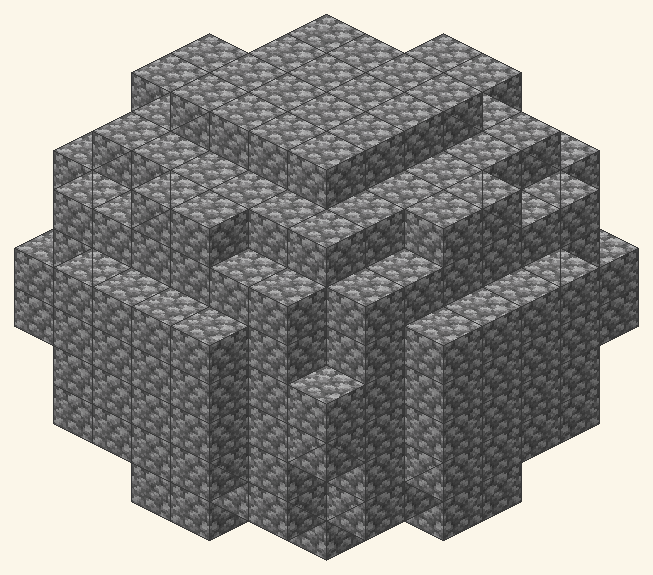
\includegraphics[width=0.55\linewidth]{fig10_3d_sphere_d12.png}\\[0.4em]
    {\sffamily\footnotesize\color{muted}A diameter-10 sphere voxelized by Block Round, rendered with the Minecraft \emph{cobblestone} texture.}
  \end{minipage}
  \vspace{0.7cm}\\
  {\color{rule}\rule{0.6\textwidth}{0.6pt}\par}
  \vspace{0.9cm}
  \begin{minipage}{0.82\textwidth}
    \centering\sffamily\small\color{muted}
    \textbf{Integrated areas:} Mathematics $\cdot$ Arts (digital art, design) $\cdot$ Computer Science $\cdot$ Digital Literacy $\cdot$ Game-based learning \\[0.4em]
    \textbf{Alignment:} Common Core State Standards (CCSS) $\cdot$ AP Calculus AB/BC $\cdot$ AP Precalculus $\cdot$ SAT/ACT Math $\cdot$ ISTE Standards $\cdot$ \hyperref[sec:olympiad]{AMC 10/12} $\cdot$ Minecraft Education
  \end{minipage}
\end{titlepage}

% =============================================================================
\renewcommand{\contentsname}{\color{accent}Contents}
\tableofcontents
\thispagestyle{fancy}
\newpage

% =============================================================================
\section{Identification and context}\label{sec:identification}

\begin{center}
\begin{tabular}{@{}p{0.32\textwidth}p{0.62\textwidth}@{}}
\toprule
\textbf{Subject area} & Mathematics (with strong interdisciplinary articulation: Arts, Computer Science, Engineering, History, Geography). \\
\addlinespace[2pt]
\textbf{Grade level} & High school --- Grade 12 (senior year). Adaptable for Grade 11 and for adult education (GED preparation, HiSET, ABE). \\
\addlinespace[2pt]
\textbf{Course types served} & Standard mathematics (Algebra 2 / Precalculus / Geometry capstone), AP Precalculus, AP Calculus AB/BC, IB Math AA/AI, Career and Technical Education (CTE) pathways, STEM magnet courses, dual-credit/early-college programs. \\
\addlinespace[2pt]
\textbf{Total instructional time} & 5 lessons of 50 minutes each (250 min in class) + optional extension activities. Block scheduling variant (two 100-min blocks + one 50-min) described in §\ref{sec:adapt}. \\
\addlinespace[2pt]
\textbf{Core resource} & Block Round --- free \emph{web} application, no account required, no server-side processing, runs offline in the browser (PWA). FERPA- and COPPA-compliant: collects no personal data and transmits nothing. Runs on low-cost \emph{smartphones} --- no Java, no Minecraft installation required. \\
\addlinespace[2pt]
\textbf{CCSS Conceptual Categories} & Geometry $\cdot$ Functions $\cdot$ Modeling $\cdot$ Number and Quantity. ISTE Standards for digital literacy. \\
\addlinespace[2pt]
\textbf{Pathway alignment} & \emph{College and career readiness} (ESSA framework); AP Computer Science Principles and AP Computer Science A; Project Lead The Way (PLTW) Engineering and Computer Science pathways; CTE Information Technology and Engineering clusters. \\
\addlinespace[2pt]
\textbf{Articulations} & \hyperref[sec:olympiad]{AMC 10/12} (Mathematical Association of America) $\cdot$ USACO (USA Computing Olympiad) $\cdot$ Science Olympiad $\cdot$ FIRST Robotics $\cdot$ Minecraft Education Edition (Microsoft Education). \\
\addlinespace[2pt]
\textbf{Student prerequisites} & Cartesian coordinate system; equation of the circle (Geometry); area and volume of elementary solids (Geometry); function notation; ratio and percent. Familiarity with \emph{Minecraft} is recommended but not required; the \emph{Block Round} software dispenses with it. \\
\addlinespace[2pt]
\textbf{Teacher preparation} & 20 minutes of prior exploration of Block Round; reading of \texttt{docs\_math/Block\_Round\_Math\_en-US.pdf} (companion technical document); optionally, light contact with \cmd{/fill}, \cmd{/clone}, and \cmd{//sphere} commands of Minecraft Java Edition. \\
\bottomrule
\end{tabular}
\end{center}

\begin{note}[Diversity of U.S. public schools]
This sequence was designed for the plural context of American Grade 12 mathematics: the large urban public high school (LAUSD, NYC DOE, Chicago Public Schools, Houston ISD); the suburban high school in mid-size cities; the rural Title I school; the STEM magnet school or Career and Technical Education (CTE) center; the Bureau of Indian Education (BIE) tribal school; the alternative high school serving over-age and under-credited students; the GED preparation program in adult education. Each context calls for specific adjustments, mapped in §\ref{sec:adapt}. Block Round was chosen because it \emph{serves all of them}: it runs on a low-cost \emph{smartphone}, requires no internet after the first load (PWA), needs no account or login, and collects no personal data --- a condition required by FERPA and COPPA.
\end{note}

\begin{minecraft}[Why anchor the sequence in Minecraft]
Minecraft is the best-selling video game in history (over 300 million copies sold). In the United States it is a transversal cultural reference among teens across every region and socioeconomic group, crossing income barriers that other video games rarely manage (the Pocket Edition for mobile costs around \$7, and \emph{Minecraft Education Edition} is free for K--12 schools through Microsoft Education). Research by the Entertainment Software Association (ESA) and Pew Research Center consistently ranks Minecraft among the top three games cited by American teenagers in every region of the country. \emph{Anchoring the sequence in Minecraft is not a passing fad: it is recognizing where American youth already live and already do geometry.}
\end{minecraft}

% =============================================================================
\section{Pedagogical rationale}\label{sec:rationale}

The choice of Block Round as a didactic artifact for Grade 12 responds to a \acc{fivefold demand} of contemporary U.S. education: integrating formal mathematics and digital literacy (a goal of the ISTE Standards and the CSTA K--12 Computer Science Framework); contextualizing abstract knowledge in practices that are \emph{meaningful} to the student; preparing for spatial geometry and function items recurring on the SAT, ACT, and AP exams; aligning with the Every Student Succeeds Act (ESSA, 2015) framework and state high school graduation requirements in the \emph{Math and Technology} domain, especially in advanced/honors pathways; and mobilizing the cultural universe of the video game \emph{Minecraft} as a motivational bridge without sacrificing mathematical rigor.

\emph{Voxel art} occupies a central place in contemporary American teen imagination. \emph{Minecraft} --- a game born in 2009, acquired by Microsoft in 2014 for \$2.5~billion, today running in classrooms through \emph{Minecraft Education Edition} --- is the most transversal cultural reference for American adolescents. Taking voxel construction as a starting point transforms a familiar \emph{ludic} tradition into a \emph{genuine mathematical problem}: how to describe, on a discrete grid of $1\times1\times1$ blocks, shapes analytically defined over $\mathbb{R}^3$. The student who builds cubes, towers, round farms, and domes every day on the community server discovers that what they already do intuitively has a formal name: \emph{voxelization}, \emph{discrete rasterization}, \emph{implicit equation of the ellipsoid}.

This pedagogical movement operates in dialogue with several traditions of educational thought widely cited in U.S. classrooms:

\begin{itemize}[leftmargin=1.3em,itemsep=0.2em,topsep=0.3em]
  \item \acc{John Dewey} (\emph{Democracy and Education}, 1916; \emph{Experience and Education}, 1938). The starting point is the student's concrete digital culture --- not the abstract equation --- which connects the sequence to Dewey's notion of \emph{experiential learning} and his motto \enquote{learning by doing}. The collaborative construction of the \enquote{membership criterion} concept is what Dewey called \emph{reflective inquiry}. The fact that the student \emph{already knows} how to build spheres in Minecraft (even intuitively) places them as an active subject, not a blank slate.

  \item \acc{Seymour Papert} (\emph{Mindstorms: Children, Computers, and Powerful Ideas}, 1980). Papert's \emph{constructionism} --- learning by making personally meaningful artifacts --- is the direct ancestor of Minecraft pedagogy. The LEGO/Logo paradigm of the MIT Media Lab anticipates by three decades the educational use of Minecraft. Papert's argument that mathematics is best learned by building \emph{things} rather than memorizing rules is realized here in literal form: every student builds, by hand and by algorithm, the mathematical objects under study.

  \item \acc{Jo Boaler} (\emph{Mathematical Mindsets}, 2015; Stanford YouCubed). Boaler's growth mindset and \emph{open mathematics} approach align with the multi-algorithm presentation of Block Round: there is not \emph{one right way} to draw a discrete circle, and that very multiplicity is itself a mathematical object. Students experience that mathematics is creative and visual, not procedural and rigid.

  \item \acc{Alan Schoenfeld} (UC Berkeley; \emph{Mathematical Problem Solving}, 1985). Schoenfeld's emphasis on \emph{metacognition} during problem-solving frames the comparative analysis of the three algorithms: students must \emph{watch themselves think} as they choose between Euclidean, Bresenham, and Threshold criteria, justifying their decisions both mathematically and aesthetically.

  \item \acc{Ubiratan D'Ambrosio} (\emph{Ethnomathematics: A Link Between Traditions and Modernity}; ICMI Felix Klein Award, 2005) and \acc{Marcia Ascher} (\emph{Ethnomathematics: A Multicultural View of Mathematical Ideas}, 1991). Different cultures construct different \enquote{ways of doing} mathematics. The three Block Round algorithms (Euclidean, Bresenham, Threshold) can be read as three distinct ethnomathematical approaches to the same problem; the circular construction tutorials popular in English-language Minecraft communities (Pixlriffs, ilmango, Mumbo Jumbo, Grian, Etho, Hermitcraft) constitute a \emph{fourth} vernacular ethnomathematics --- popular, oral, game-mediated, contemporary.

  \item \acc{Lev Vygotsky} (\emph{Mind in Society}, posthumous 1978; Zone of Proximal Development). Cooperative pair/trio work in the activities operates within the ZPD: the student who already builds spheres in Minecraft and the student who has never played meet at the algorithm, and each learns from the other.
\end{itemize}

The software fulfills a precise epistemic function: it \emph{does not replace} algebra, but \emph{materializes} the difference between competing mathematical formulations. The three algorithms correspond to three mathematically distinct definitions of the same object --- the discrete circle --- and produce visibly different drawings, as illustrated in Figure~\ref{fig:comp-d10}. The student perceives, with their own eyes, that \emph{the definition matters}, and simultaneously that the result is not abstract: \emph{they can build it, block by block, in Minecraft}.

\begin{figure}[!htbp]
\centering
\begin{subfigure}[t]{0.31\linewidth}\centering
  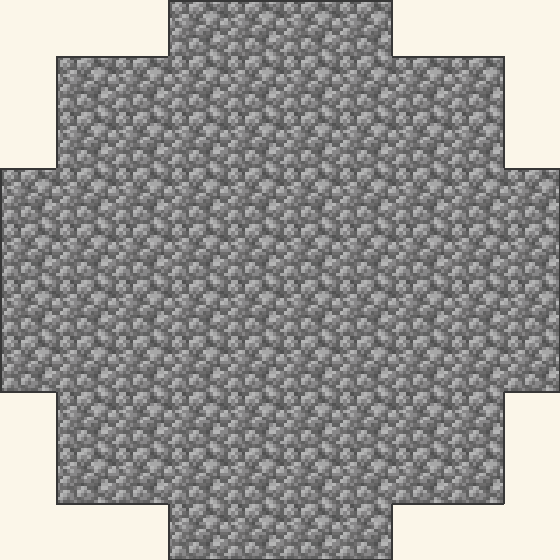
\includegraphics[width=\linewidth]{fig01_2d_d10_euclidean.png}
  \caption{\emph{Euclidean}}
\end{subfigure}\hfill
\begin{subfigure}[t]{0.31\linewidth}\centering
  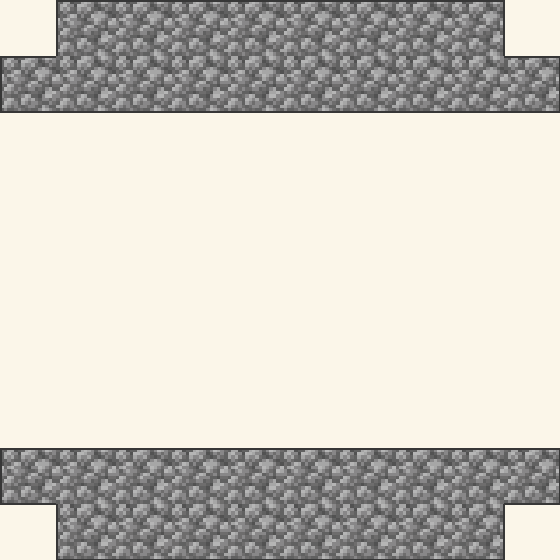
\includegraphics[width=\linewidth]{fig02_2d_d10_bresenham.png}
  \caption{\emph{Bresenham}}
\end{subfigure}\hfill
\begin{subfigure}[t]{0.31\linewidth}\centering
  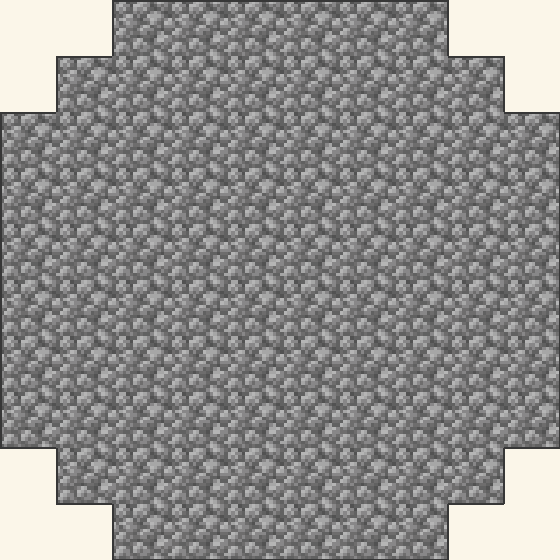
\includegraphics[width=\linewidth]{fig03_2d_d10_threshold.png}
  \caption{\emph{Threshold}}
\end{subfigure}
\caption{The same circle of diameter 10 under three membership criteria, rendered with the Minecraft \emph{cobblestone} texture. Notice how the corner cell, the line-to-line transition, and the cardinal points vary --- three responses that are \emph{mathematically correct} under different criteria, and three different construction plans in \emph{Minecraft}.}
\label{fig:comp-d10}
\end{figure}

\begin{note}[Equity and the material reality of U.S. public schools]
The choice of Block Round responds, in part, to a concrete material problem: the inequality of access to digital resources across American public schools. The 2023 NAEP and NCES reports document persistent gaps in technology access, particularly along lines of district funding and rural geography. The \emph{digital divide} highlighted by Pew Research and Common Sense Media remains very real --- not every school has a one-to-one Chromebook program, and \$4B+ in ESSER (Elementary and Secondary School Emergency Relief) funding only partially closed the gap. On the other hand, smartphone ownership among adolescents aged 15--17 exceeds 95\% (Pew Research, 2023). Block Round was designed for exactly that scenario: low-cost \emph{smartphone}, no permanent internet, no account --- and, when needed, Appendix~\ref{ap:adapt-analog} offers a \emph{fully analog} itinerary using only graph paper. \emph{Minecraft Pocket Edition itself runs on three-year-old phones}: a student can start with Block Round in class and continue at home in Minecraft.
\end{note}

\begin{minecraft}[Research: Minecraft in American education]
American research has documented Minecraft's pedagogical use across many districts. Authors such as Karen Schrier (\emph{Knowledge Games}, Johns Hopkins University Press), Constance Steinkuehler (UC Irvine, Connected Learning Research Network), Kurt Squire (UC Irvine, \emph{Video Games and Learning}), and the MIT Education Arcade have documented Minecraft use in mathematics, programming, and STEM project-based learning. Microsoft Education maintains a comprehensive repository of lesson plans in English at the \emph{Minecraft Education Edition} portal (\url{https://education.minecraft.net}). This sequence complements that tradition: it uses Block Round as a \emph{bridge} to Minecraft, dispensing with game installation (and the associated license, Java, or Microsoft account requirements) at the moment of the class.
\end{minecraft}

% =============================================================================
\section{Learning objectives}\label{sec:objectives}

\subsection{Overarching objective}

To lead students to \acc{understand, compare, use, and translate-into-construction} the formal definitions of the circle, the ellipse, and the ellipsoid as criteria for cell inclusion on a discrete grid of textured voxels, mobilizing the implicit equation of these figures to explain, predict, modify, and \emph{build in Minecraft} authorial visual productions, in dialogue with American visual heritage (modernist and minimalist art, Indigenous architectural traditions, geometric ceramics of Mound Builder and Pueblo cultures) and with the contemporary American mathematical tradition. Awareness of this multiplicity of valid responses connects to a U.S. mathematical culture in which Maryam Mirzakhani (Stanford, Fields Medal 2014) became the first woman ever to receive the highest honor in mathematics, and to a gaming culture in which American Minecraft communities build entire cities, articulating spatial geometry daily without necessarily naming it.

\subsection{Specific objectives}

\textbf{Cognitive (conceptual):}
\begin{itemize}[leftmargin=1.3em,itemsep=0.2em,topsep=0.3em]
  \item identify the implicit equation $\left(\dfrac{x}{r_x}\right)^{\!2} + \left(\dfrac{y}{r_y}\right)^{\!2} = 1$ as the general case containing the circle $x^2 + y^2 = r^2$;
  \item recognize that three different membership criteria (distance from center, Bresenham midpoint, corner coverage) produce three distinct sets of cells --- as seen in Figure~\ref{fig:comp-d10};
  \item understand the transition from the 2D equation to the 3D equation of the ellipsoid and relate it to the volume formula $V = \tfrac{4}{3}\pi r_x r_y r_z$ (a recurring topic on the SAT Math Geometry section and AP Calculus volume of solids of revolution);
  \item interpret the cutting of a solid by a plane as a \emph{linear inequality} applied to voxel coordinates;
  \item understand the \emph{arithmetic of the Minecraft inventory} (stacks of 64, single chests of 27 slots, double chests of 54 slots) as a concrete application of \emph{ceiling division} and \emph{representation of quotient and remainder};
  \item identify the \emph{symmetries} (reflection, rotation) that allow a complete sphere to be built from one octant via \cmd{/clone}.
\end{itemize}

\textbf{Procedural:}
\begin{itemize}[leftmargin=1.3em,itemsep=0.2em,topsep=0.3em]
  \item operate the Block Round interface in both modes (2D and 3D) and export PNG images and \texttt{.schem} schematics;
  \item hand-draw, on graph paper, the discrete approximation of a circle applying the Euclidean criterion and verify it against the software output;
  \item compute the discrete area/volume of a voxelized figure by counting cells and compare with the continuous area/volume, expressing the result as relative error;
  \item compose an authorial figure combining circles, ellipses, and ellipsoids with mathematical justification for the choices, predicting the number of blocks per type and the number of double chests required;
  \item import a schematic exported by Block Round into Litematica or Schematica (Minecraft mods) and execute the construction in-game;
  \item write a sequence of \cmd{/clone} commands that reflects one octant into a complete sphere.
\end{itemize}

\textbf{Attitudinal:}
\begin{itemize}[leftmargin=1.3em,itemsep=0.2em,topsep=0.3em]
  \item cooperate in pairs or trios on practical activities, simulating Minecraft server \emph{builder} teams;
  \item argue mathematically in defense of an aesthetic choice --- a skill directly assessed in AP exam free-response items and in oral defenses for research competitions;
  \item recognize that real problems (including the problem of \enquote{building a Quartz dome on the class server}) admit more than one technically correct response;
  \item identify mathematical references in American cultural heritage, in Indigenous traditional knowledge, and in contemporary digital production (server builders, streamers, Minecraft networks);
  \item develop \emph{digital ethics}: respect peer work, credit reused builds, and understand the concept of software license (open source vs.\ proprietary).
\end{itemize}

% =============================================================================
\section{Standards alignment}\label{sec:standards}

The sequence directly mobilizes \acc{four high school standards} from the Common Core State Standards (CCSS) for Mathematics, plus articulations with the Next Generation Science Standards (NGSS) cross-cutting concepts, the ISTE Standards for Students, and the CSTA K--12 Computer Science Framework.

\begin{standard}[CCSS.MATH.CONTENT.HSG.GMD.A.3]
Use \acc{volume formulas for cylinders, pyramids, cones, and spheres} to solve problems. (Directly aligned with the volume of the discrete ellipsoid computed in Lesson 3 and Lesson 4.)
\end{standard}

\begin{standard}[CCSS.MATH.CONTENT.HSG.GPE.A.1]
\acc{Derive the equation of a circle} of given center and radius using the Pythagorean Theorem; complete the square to find the center and radius of a circle given by an equation. (Directly aligned with the implicit equation introduced in Lesson 1.)
\end{standard}

\begin{standard}[CCSS.MATH.CONTENT.HSF.IF.B.4]
For a function that models a relationship between two quantities, interpret key features of graphs and tables in terms of the quantities, and sketch graphs showing key features given a verbal description of the relationship. (Aligned with multiple representations of the discrete circle: algebraic, graphical, voxel-grid.)
\end{standard}

\begin{standard}[CCSS.MATH.CONTENT.HSG.MG.A.3]
Apply \acc{geometric methods to solve design problems} (e.g., designing an object or structure to satisfy physical constraints or minimize cost). (Directly aligned with the optimization activities in Lesson 4: stacks, chests, octahedral symmetry to minimize block placement.)
\end{standard}

\medskip
The sequence also engages the eight \emph{Standards for Mathematical Practice}:

\begin{itemize}[leftmargin=1.3em,itemsep=0.15em,topsep=0.3em]
  \item \acc{MP1} --- Make sense of problems and persevere in solving them;
  \item \acc{MP3} --- Construct viable arguments and critique the reasoning of others (essential for the defense of algorithmic choices in Lesson 5);
  \item \acc{MP4} --- Model with mathematics (entire sequence);
  \item \acc{MP5} --- Use appropriate tools strategically (Block Round, Minecraft, graph paper);
  \item \acc{MP6} --- Attend to precision (especially in stack/chest arithmetic of Lesson 4).
\end{itemize}

\subsection{Alignment with AP Calculus, AP Precalculus, SAT, and ACT}\label{sec:ap}

The standards above connect with the following exam frameworks:

\begin{itemize}[leftmargin=1.3em,itemsep=0.15em,topsep=0.3em]
  \item \acc{AP Calculus AB/BC} --- Unit 8 (Applications of Integration), specifically \emph{Volumes of Solids of Revolution} (disk and shell methods), \emph{Volumes with Known Cross-Sections}, and \emph{Riemann sums as discretization} --- the same conceptual move underlying voxelization.
  \item \acc{AP Precalculus} (since 2023) --- Unit 1 (Polynomial and Rational Functions), Unit 3 (Trigonometric Functions, including the unit circle), and the implicit-curve framework.
  \item \acc{SAT Math} --- the \emph{Geometry and Trigonometry} cluster (volume formulas, equation of a circle, coordinate geometry), plus \emph{Problem Solving and Data Analysis} (ratios, percent error from discrete-vs-continuous volume).
  \item \acc{ACT Math} --- the \emph{Plane Geometry} and \emph{Coordinate Geometry} subscores; specifically items on circle equations, volumes, and proportional reasoning.
  \item \acc{AP Computer Science Principles} --- Big Ideas 3 (Algorithms and Programming) and 4 (Computer Systems and Networks); Bresenham's algorithm is a classic case study.
\end{itemize}

The College Board portal (\url{https://apcentral.collegeboard.org}) provides exam frameworks and released items for further alignment work.

\subsection{Digital literacy and the ISTE Standards}

The ISTE Standards for Students (especially the \emph{Computational Thinker} and \emph{Creative Communicator} strands) frame the digital-literacy aspect of the sequence. Discussions of \emph{digital ethics} (open-source vs.\ proprietary licensing; Mojang/Microsoft permits free educational use of Minecraft through \emph{Education Edition}), \emph{data privacy} (\href{https://studentprivacy.ed.gov/}{FERPA}, COPPA), \emph{authorial production} (rights over student creations in Lesson~\ref{lesson5}), and \emph{digital citizenship} (responsible behavior on Minecraft servers, prevention of \emph{griefing} and online bullying) run throughout the sequence.

% =============================================================================
\section{Content}\label{sec:content}

\subsection{Conceptual}
\begin{itemize}[leftmargin=1.3em,itemsep=0.15em,topsep=0.3em]
  \item Cartesian coordinate system in $\mathbb{R}^2$ and $\mathbb{R}^3$; cell center \emph{vs.} corner.
  \item Standard equation of the circle: $x^2 + y^2 = r^2$.
  \item General implicit equation of the ellipse: $\left(\dfrac{x}{r_x}\right)^{\!2} + \left(\dfrac{y}{r_y}\right)^{\!2} = 1$.
  \item Membership inequality: \emph{interior, exterior,} and \emph{boundary}.
  \item Equation of the ellipsoid and sphere in $\mathbb{R}^3$.
  \item Continuous volume of the ellipsoid: $V = \tfrac{4}{3}\pi r_x r_y r_z$.
  \item Planes in space as linear inequalities (cutting operation).
  \item Cell neighborhoods (4-connected in 2D, 6-connected in 3D).
  \item \acc{Minecraft inventory arithmetic}: stacks of 64; single chests (27 slots) and double chests (54 slots); ceiling division $N_{\mathrm{stacks}} = \lceil N/64 \rceil$.
  \item \acc{Octahedral symmetry} and the $\mathbb{Z}_2^3$ group of coordinate reflections (an order-8 subgroup of $O_h$): application to optimized construction via \cmd{/clone}.
\end{itemize}

\subsection{Procedural}
\begin{itemize}[leftmargin=1.3em,itemsep=0.15em,topsep=0.3em]
  \item Hand-drawing on graph paper following an explicit criterion.
  \item Operating Block Round (mode switching, slider adjustment, algorithm choice, export as PNG and \texttt{.schem}).
  \item Comparing discrete and continuous areas/volumes by counting.
  \item Composing combined figures (authorial \emph{voxel art} with geometric justification).
  \item Importing \texttt{.schem} into Litematica/Schematica.
  \item Executing vanilla commands \cmd{/fill}, \cmd{/clone}, \cmd{/setblock}, and WorldEdit \cmd{//sphere}, \cmd{//hsphere}, \cmd{//ellipsoid}.
  \item Planning resource collection in survival mode.
\end{itemize}

\subsection{Attitudinal}
\begin{itemize}[leftmargin=1.3em,itemsep=0.15em,topsep=0.3em]
  \item Cooperative work in pairs or trios.
  \item Reasoned argumentation (justifying choices with mathematics).
  \item Digital ethics: respect for the software license, for peer productions, and for shared Minecraft server rules.
  \item Appreciation of mathematical references present in American cultural heritage, Indigenous traditional knowledge, and contemporary \emph{gamer} culture.
\end{itemize}

\subsection{Rendering modes and algorithmic variety}

In addition to changing algorithms, Block Round offers three \emph{rendering modes} (Filled, Thin, Thick) that produce distinct visuals for the same geometric figure, as illustrated in Figure~\ref{fig:render-modes}. In Minecraft, these modes correspond to three different construction types: a \emph{Filled} sphere uses all interior blocks (an opaque \emph{Stone} dome); \emph{Thin} shows only the shell (a \emph{hollow} dome, internally empty for a hall or museum); \emph{Thick} closes the diagonal seams that the Thin mode leaves (\emph{essential} for underwater \emph{Glass} or \emph{Ice} domes that must be watertight).

\begin{figure}[!htbp]
\centering
\begin{subfigure}[t]{0.31\linewidth}\centering
  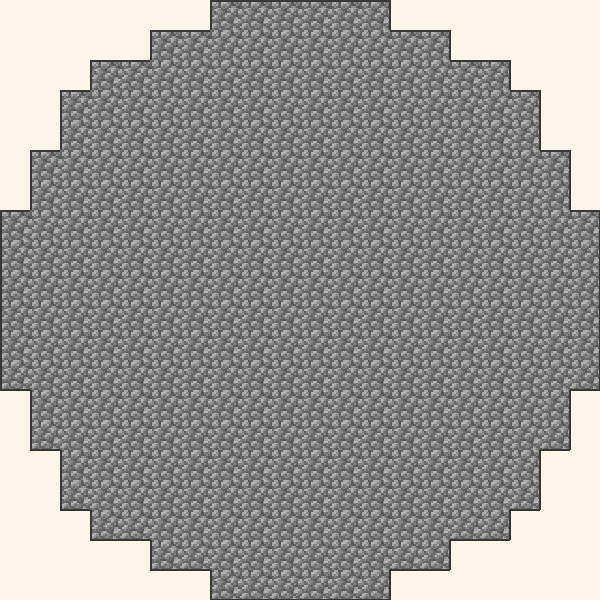
\includegraphics[width=\linewidth]{fig04_2d_d20_euclidean.png}
  \caption{\emph{Filled}}
\end{subfigure}\hfill
\begin{subfigure}[t]{0.31\linewidth}\centering
  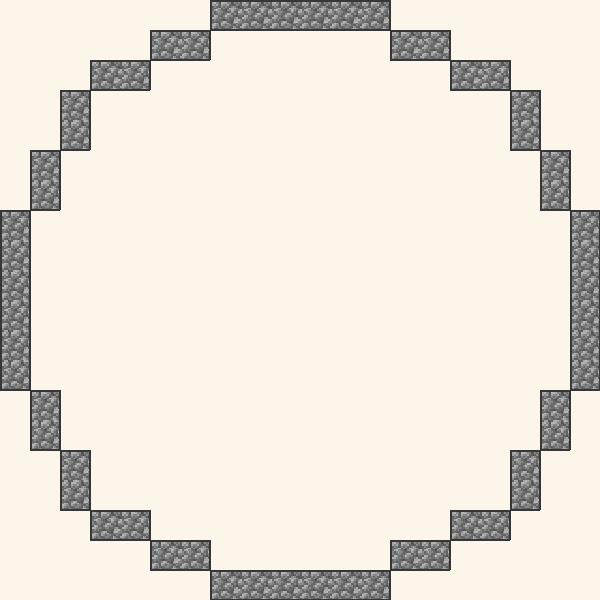
\includegraphics[width=\linewidth]{fig08_2d_d20_thin.png}
  \caption{\emph{Thin} (1-block outline)}
\end{subfigure}\hfill
\begin{subfigure}[t]{0.31\linewidth}\centering
  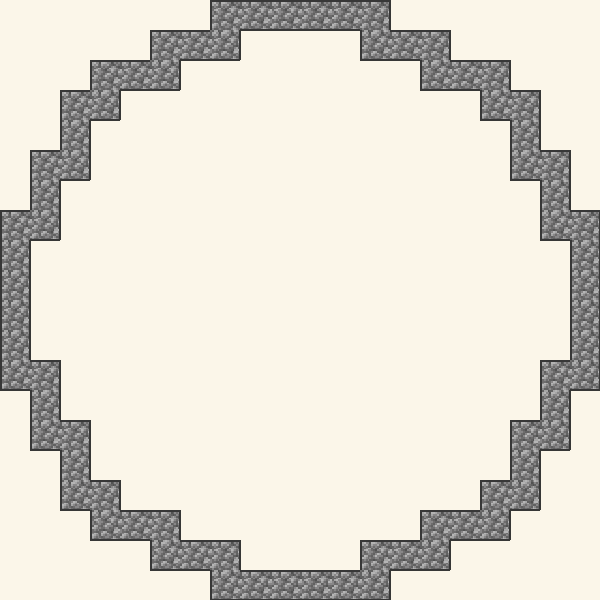
\includegraphics[width=\linewidth]{fig09_2d_d20_thick.png}
  \caption{\emph{Thick} (outline with diagonal bridges)}
\end{subfigure}
\caption{The three rendering modes for the same Euclidean circle of diameter 20. The \emph{Thin} mode corresponds to the topological discrete boundary; the \emph{Thick} mode adds blocks at the diagonals to avoid $45^\circ$ holes --- exactly the problem that appears in an underwater Glass dome in Minecraft, where a diagonal seam lets water leak in.}
\label{fig:render-modes}
\end{figure}

\subsection{Block textures: the Block Round differential}

While the mathematics of \emph{which voxels to place} is texture-independent, Block Round renders each voxel with its canonical six-face Minecraft texture. The same diameter-10 sphere completely changes character depending on the chosen block (Figure~\ref{fig:textures}), \emph{with no change to the underlying algorithm}. This is the central pedagogical point: \emph{form} is a product of mathematics; \emph{appearance} is a subsequent aesthetic decision.

\begin{figure}[!htbp]
\centering
\begin{subfigure}[t]{0.31\linewidth}\centering
  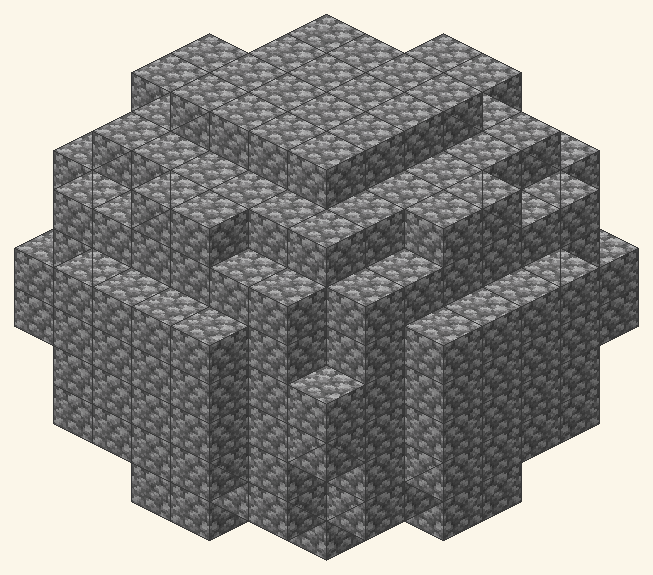
\includegraphics[width=\linewidth]{fig15_3d_sphere_cobblestone.png}
  \caption{\emph{Cobblestone}}
\end{subfigure}\hfill
\begin{subfigure}[t]{0.31\linewidth}\centering
  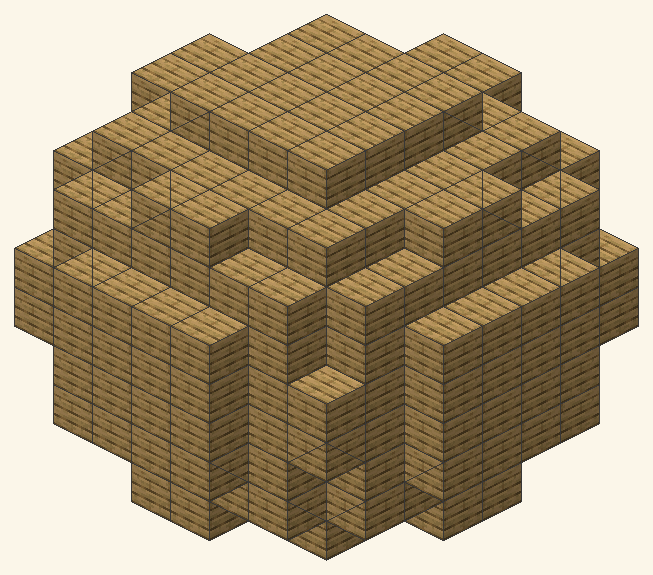
\includegraphics[width=\linewidth]{fig17_3d_sphere_oak.png}
  \caption{\emph{Oak Planks}}
\end{subfigure}\hfill
\begin{subfigure}[t]{0.31\linewidth}\centering
  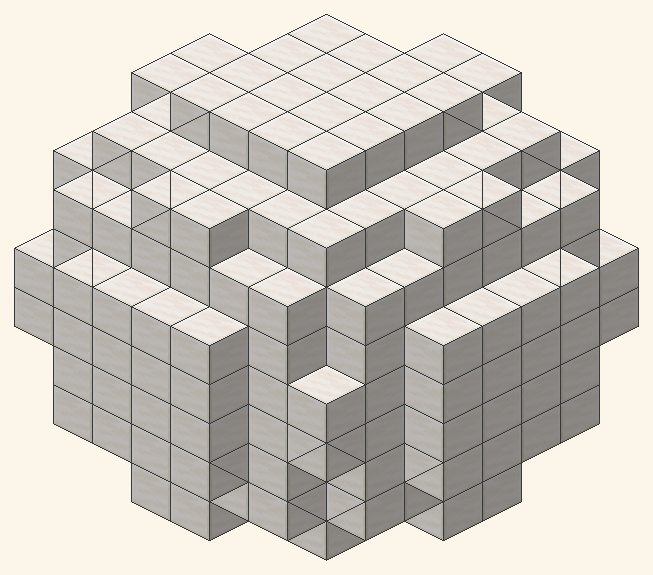
\includegraphics[width=\linewidth]{fig19_3d_sphere_quartz.png}
  \caption{\emph{Quartz Block}}
\end{subfigure}
\caption{Three Minecraft textures applied to the \emph{same} diameter-10 sphere. The voxelized silhouette is identical across the three versions --- the mathematics has not changed. What changes is visual character: \emph{Cobblestone} suggests medieval walls, \emph{Oak Planks} suggests cabin or ship interior, \emph{Quartz Block} suggests modern temple.}
\label{fig:textures}
\end{figure}

% =============================================================================
\section{Prerequisites}\label{sec:prerequisites}

The sequence presupposes prior contact with:

\begin{itemize}[leftmargin=1.3em,itemsep=0.15em,topsep=0.3em]
  \item Cartesian coordinate system: locating points $(x, y)$ and $(x, y, z)$.
  \item Standard equation of the circle (typically covered in Geometry, Grade 10).
  \item Areas of polygons and the circle; volumes of cube, prism, and cylinder (Geometry).
  \item Concept of function: domain, range, graph.
  \item Notion of ratio and percent.
  \item Integer division with quotient and remainder (Grade 6--7).
\end{itemize}

\emph{Optional prior knowledge (not required, but useful):} familiarity with Minecraft. This sequence was deliberately designed so that even students who have \emph{never} played Minecraft (a rare situation but possible, especially in some rural schools with limited connectivity) can fully follow along --- all operations happen in Block Round, which is \emph{self-contained} in the browser.

If the class shows gaps in any of the required prerequisites above --- a frequent reality in the post-pandemic context, as documented by the 2022 NAEP results showing significant declines in mathematics scores nationwide --- \emph{Lesson 1} includes a \emph{diagnostic review} moment (10 min) described in §\ref{lesson1}.

% =============================================================================
\section{Resources and materials}\label{sec:resources}

\subsection{Digital resources}
\begin{itemize}[leftmargin=1.3em,itemsep=0.15em,topsep=0.3em]
  \item Block Round (one instance per student \emph{or} per pair);
  \item Multimedia projector, HDMI-equipped TV, or interactive whiteboard (SMART Board, Promethean, etc.);
  \item Access to a \emph{computer lab} \emph{or} use of personal \emph{smartphones} (BYOD --- \emph{Bring Your Own Device}) \emph{or} school-provided \emph{Chromebooks/tablets} (1:1 programs);
  \item (Optional, Lesson~\ref{lesson5}) access to Minecraft Java Edition or Minecraft Education Edition with \emph{Litematica} or \emph{Schematica} mods installed; alternatively, vanilla use with \cmd{/fill} and \cmd{/clone}.
\end{itemize}

\subsection{Analog resources}
\begin{itemize}[leftmargin=1.3em,itemsep=0.15em,topsep=0.3em]
  \item Graph paper (1/4 inch or 1 cm), 2 sheets per student;
  \item Pencil, eraser, 12-inch (30-cm) ruler;
  \item Colored pencils or markers (preferably grass-green \texttt{\#5B8E3F} and dirt-brown \texttt{\#825432}, the Block Round palette);
  \item Exercise handout (Appendix~\ref{ap:exerc});
  \item Whiteboard or chalkboard.
\end{itemize}

\subsection{Textbook alignment}\label{sec:textbook}

Block Round complements --- it does not replace --- the mathematics textbook adopted by the school. Commonly adopted Grade 12 textbooks that cover the content engaged here:

\begin{itemize}[leftmargin=1.3em,itemsep=0.1em,topsep=0.2em,nosep]
  \item \emph{Precalculus} (Larson, Hostetler), Cengage;
  \item \emph{Precalculus: Mathematics for Calculus} (Stewart, Redlin, Watson), Cengage;
  \item \emph{Calculus: Early Transcendentals} (Stewart), Cengage --- for AP Calculus connections;
  \item \emph{Geometry} (Holt McDougal / Houghton Mifflin Harcourt) --- for sphere/ellipsoid volume foundations;
  \item \emph{Big Ideas Math: Algebra 2} (Larson, Boswell) --- a Common Core-aligned series widely adopted;
  \item \emph{enVision Mathematics} (Pearson / Savvas Learning Company).
\end{itemize}

The chapters on \emph{equation of the circle}, \emph{conic sections}, and \emph{three-dimensional measurement} (volumes) dialogue directly with this sequence. In particular, problems of \emph{tiling}, \emph{coverage}, and \emph{counting on a grid} (common in U.S. high school textbooks) are nearly identical to the central problem of Block Round, just with different terminology.

\subsection{Accessing Block Round}

In order of preference:

\begin{enumerate}[leftmargin=1.5em,itemsep=0.15em,topsep=0.3em]
  \item \textbf{Teacher-hosted} on \emph{GitHub Pages} or the school portal (URL distributed via QR Code projected on the board). Public version: \url{https://vinisouza128.github.io/block-round/}.
  \item \textbf{Local copy} of the project files in a lab folder, executed via \emph{file://}.
  \item \textbf{Offline on \emph{smartphone}} via PWA: simply open once with internet so the browser can install the app.
\end{enumerate}

% =============================================================================
\section{Adaptations for the plural reality of U.S. schools}\label{sec:adapt}

The American public school system is heterogeneous --- across state lines, district lines, and within a single district. This sequence was designed to adapt to that plurality, with specific variants for each context.

\subsection{Large urban public high school}
Typical scenario of LAUSD (Los Angeles), NYC DOE (New York City), Chicago Public Schools (CPS), Houston ISD, Philadelphia SDP, Miami-Dade County Public Schools. Generally features computer labs (shared use), smartboards, and decent Wi-Fi. Many districts already license \emph{Minecraft Education Edition} for students through their Microsoft 365 EDU subscription --- Lesson~\ref{lesson5} can be done entirely in that version. \emph{The most straightforward configuration for implementing the sequence fully in a lab setting.}

\subsection{Suburban or mid-size city public high school}
The reality of much of suburban America. Computer labs may exist but be heavily booked. Recommended \emph{BYOD model} with personal student smartphones, organized in pairs (one phone per pair). Block Round runs comfortably on Android phones from 2018 onward and any iPhone 8 or newer. If \emph{Minecraft} is unavailable, Lesson~\ref{lesson5} can focus on hypothetical commands (paper + description of effect) without losing conceptual content. This is the \acc{most common} configuration nationwide.

\subsection{Rural Title I school}
A reality across the rural United States --- Appalachian school districts, the Great Plains, the Mississippi Delta, frontier schools in Wyoming, Montana, and Alaska, and the few remaining one-room schoolhouses. Often less equipped digitally but with \emph{strong prior geometric knowledge} from students (geometry applied to fields, fencing, contour irrigation, livestock pens). The analog variant (Appendix~\ref{ap:adapt-analog}) and a single teacher device for demonstration are recommended. Lesson~\ref{lesson3} can leverage students' knowledge of constructing circular livestock pens, silos, and grain bins to articulate lived geometry and symbolic geometry.

\subsection{Career and Technical Education (CTE) and STEM magnet schools}
Specialized U.S. high schools such as Stuyvesant, Bronx Science, and Brooklyn Tech (NYC), TJHSST (Thomas Jefferson High School for Science and Technology, Virginia), Bergen County Academies (NJ), or Project Lead The Way (PLTW)-network schools, P-TECH (Pathways in Technology Early College HS) programs. Generally very well equipped. The sequence integrates naturally with CTE pathways in \emph{Information Technology}, \emph{Engineering and Architecture}, \emph{Computer Programming}, \emph{Digital Arts and Design}, and \emph{Mechatronics}. It is recommended to deepen Lesson~\ref{lesson2} (Bresenham's algorithm) with a Python implementation in the lab, and Lesson~\ref{lesson5} with the actual installation of a Minecraft Java server in the lab for collaborative construction --- a frequent activity in CTE Information Technology programs. The sequence articulates with computer-science course frameworks at schools participating in \emph{Code.org}, \emph{AP CSP}, and the \emph{Computer Science for All} initiative.

\subsection{Schools serving Indigenous students (BIE and tribal schools)}
The Bureau of Indian Education (BIE) network within the Department of Interior administers schools serving Native American students; tribally controlled schools operate under the Tribally Controlled Schools Act (1988). The Native American Languages Act (1990) and Title VI of ESEA (Indian Education) frame the curricular context. This sequence can be \emph{enriched with community-specific knowledge}: traditional Pueblo kivas (round ceremonial chambers); Plains tipi (conic geometry); the Navajo hogan (hexagonal or octagonal); the Wampanoag wetu (dome-shaped, often elliptical); the Anishinaabe wigwam. \emph{The arts teacher, the social studies teacher, and tribal elders are essential partners in this adaptation} (see Lesson~\ref{lesson3}, Activity~\ref{at:34}). State frameworks such as Montana's \emph{Indian Education for All} (Article X §1(2) of the Montana Constitution), Washington's SB 5433, and New Mexico's Indian Education Act provide additional curricular hooks. Block Round's privacy stance --- storing nothing, transmitting nothing --- aligns with Indigenous \emph{data sovereignty} principles.

\subsection{Schools in underfunded urban districts (urban Title I)}
Schools serving majority students of color in historically underfunded districts (Detroit Public Schools, Baltimore City Public Schools, Jackson Public Schools MS, Camden NJ, Birmingham AL) often have outdated lab equipment alongside surprisingly strong BYOD/smartphone access. The \$4B+ in ESSER funding has partially addressed equipment needs but maintenance and IT support remain a challenge. The Block Round + smartphone model fits well here. Equity is foregrounded by Lesson~\ref{lesson4}, where the conversation about \emph{stack arithmetic} (\enquote{how many supply chests do we need?}) translates naturally into broader conversations about resource constraints and optimization. Block Round's open access (no fees, no licenses, no required hardware beyond a phone) embodies the equity principle.

\subsection{Adult education / Alternative high schools}
Adult basic education (ABE), GED preparation, HiSET, and alternative high schools (e.g., Diploma Plus model, YouthBuild). Typically evening or hybrid classes with adult students returning to complete a high school credential. Block Round works well here because the interface is friendly and the theme (Minecraft / video games) is also familiar to this age range (many adults aged 25--40 grew up with Minecraft from 2010 onward; others learned it through their children). Suggest reducing the time of each activity by 20\% (given the shorter session length of evening classes) and prioritizing oral discussion over long written production. Lesson~\ref{lesson5} can be made \emph{optional} for adult-ed contexts, focusing on Lessons 1--4.

\subsection{Block scheduling variant (two 100-min blocks)}
For schools on block schedule (frequent in suburban high schools and in many states' high school reform models): Lessons 1+2 in one block, 3+4 in another, Lesson 5 alone (in a 50-min slot, or in a 100-min block if there's time for actual Minecraft construction). Total: three 100-min blocks + one 50-min slot, or two 100-min blocks + one double block (200 min) for the practical Minecraft construction phase.

\subsection{Crosswalk with state curriculum frameworks}

The Common Core State Standards (CCSS) have been adopted by 41 states + DC; many adopting states have modified or replaced them with their own frameworks. Major frameworks:

\begin{center}
\small
\begin{tabularx}{\textwidth}{@{}p{0.16\textwidth}p{0.26\textwidth}X@{}}
\toprule
\textbf{State} & \textbf{Framework} & \textbf{Course in which sphere/ellipsoid volumes appear} \\
\midrule
California & Common Core CA, A--G requirements & Geometry (10), Algebra 2 / Math III (11), Calculus AP (12). Smarter Balanced (SBAC) assessment. \\
\addlinespace[3pt]
Texas & TEKS (Texas Essential Knowledge and Skills) & Geometry (Math.4--5), Precalculus, AP Calculus. STAAR EOC end-of-course assessment. \\
\addlinespace[3pt]
New York & NYS Next Generation Mathematics Learning Standards & Geometry Regents, Algebra II Regents, Precalculus. Regents Exam. \\
\addlinespace[3pt]
Florida & B.E.S.T.\ Standards (post-CCSS, 2020) & Geometry, Algebra 2, Precalculus Honors. FAST (Florida Assessment of Student Thinking). \\
\addlinespace[3pt]
Massachusetts & MA Curriculum Framework for Mathematics (2017) & Geometry, Algebra 2, Precalculus. MCAS end-of-course. \\
\addlinespace[3pt]
Virginia & SOL (Standards of Learning) & Geometry, Algebra 2, Trigonometry, AP Calculus. SOL EOC assessment. \\
\bottomrule
\end{tabularx}
\end{center}

\subsection{Hybrid and remote learning}
The \emph{web-based} nature of Block Round makes it trivially compatible with remote classes (\emph{Zoom}, \emph{Google Meet}, \emph{Microsoft Teams}, Canvas/Schoology/Google Classroom). The teacher shares their screen; students follow along on their own device. Many districts continue to use hybrid models post-COVID, and the digital-divide research from Pew Research, EdWeek, and the National School Boards Association documents that this matters most for low-income students. Graph-paper activities can be photographed and submitted as asynchronous work through any LMS or via class messaging. Lesson~\ref{lesson5} can be done on a shared Minecraft server --- \emph{Realms} (Microsoft's hosted service) or a teacher-run server --- with the class meeting in the virtual world and building collaboratively.

% =============================================================================
\section{Lesson sequence}\label{sec:sequence}

The sequence follows the \acc{engagement --- problematization --- systematization --- synthesis} structure, drawing on the 5E Instructional Model (Engage, Explore, Explain, Elaborate, Evaluate) widely used in U.S. STEM education and on Dewey's reflective-inquiry tradition of starting from the student's prior knowledge. Each 50-minute lesson respects the cognitive rhythm of the high school senior, alternating brief expository moments ($\leq 15$\,min) with practical activities.

% =============================================================================
\subsection{Lesson 1 --- \enquote{How does the game draw a sphere out of cubes?}}\label{lesson1}

\subsubsection*{Lesson objective}
Establish the \emph{central problem} of discrete rasterization as a genuine mathematical problem, mobilize the equation of the circle, and introduce Block Round. Recognize that the central problem of the lesson --- \emph{how do we decide which blocks to place?} --- is exactly the problem that every Minecraft player faces when building a sphere in the game.

\begin{activity}[1.1 --- Engagement \quad\timetag{10 min}]
\textbf{Strategy:} \emph{think--pair--share} (think individually, talk in pairs, share with the class). \\[0.4em]
\textbf{Step-by-step:}
\begin{enumerate}[leftmargin=1.5em,itemsep=0.2em,topsep=0.3em,nosep]
  \item Project (or sketch) three classic Minecraft constructions: a Glass dome on a Stone base (any popular tutorial by Pixlriffs, Mumbo Jumbo, or ilmango on YouTube); the \emph{Giant Sphere} collaboratively built on a popular community server (Hermitcraft, MCC Island, Hypixel); a Minecraft pixel-art portrait of an American cultural icon (Spider-Man, Mickey Mouse, a Pokémon, an NBA logo).
  \item Ask the class: \emph{\enquote{Look closely. How does the game decide which cubes to place to make a sphere? Does Minecraft have a built-in magic compass?}}
  \item Each student writes their answer individually (1 min) and then discusses with their seat partner (2 min).
  \item Collect responses: write key ideas in the corner of the board. Steer toward the fundamental observation: \emph{\enquote{The game can only place whole cubes --- how does it decide which ones?}}
\end{enumerate}
\end{activity}

\begin{activity}[1.2 --- Problematization \quad\timetag{15 min}]
\textbf{Strategy:} hand-drawing confronted with the formal definition. \\[0.4em]
\textbf{Materials:} graph paper, pencil. \\[0.4em]
\textbf{Step-by-step:}
\begin{enumerate}[leftmargin=1.5em,itemsep=0.2em,topsep=0.3em,nosep]
  \item Each student gets half a sheet of graph paper and marks the center point of an $11 \times 11$ cell region.
  \item Instruction: \emph{\enquote{Shade the best circle you can with diameter 10 (radius 5). \emph{Imagine each square is a Minecraft cobblestone block.} You have 4 minutes.}}
  \item After the time, three or four students go to the board to reproduce their drawing on a grid drawn in chalk/marker.
  \item Teacher-directed observation: \emph{\enquote{Look. Did you make the same figure? Why not? Who is right? If each of you were building this sphere on a shared Minecraft server, what problem would this create?}}
  \item Systematize: there is no \emph{single} right answer (Figure~\ref{fig:comp-d10} shown in §\ref{sec:rationale} confirms this). Each student implicitly adopted a different \acc{criterion} for deciding whether a cell counts.
\end{enumerate}

\textbf{Ethnomathematical note:} take the opportunity to mention that \emph{this diversity of responses is exactly the object of Ethnomathematics} (Ubiratan D'Ambrosio, Marcia Ascher), a field that studies how different cultures and groups solve mathematical problems in distinct and equally valid ways. \emph{The American Minecraft community itself constitutes a cultural group with its own \enquote{ethnomathematics}}, transmitted through YouTube tutorials, mods written by community members, and servers like Hermitcraft and the MCC tournament network.
\end{activity}

\begin{activity}[1.3 --- Systematization \quad\timetag{15 min}]
\textbf{Strategy:} dialogued exposition with board support. \\[0.4em]
\textbf{Content:}

The implicit equation of the circle centered at the origin with radius $r$ is

\begin{formula}
\centering
$\displaystyle x^2 + y^2 \;=\; r^2$
\end{formula}

Points \emph{inside} satisfy $x^2 + y^2 < r^2$; points \emph{outside}, $x^2 + y^2 > r^2$. The equation generalizes to an ellipse with semi-axes $r_x, r_y$:

\begin{formula}
\centering
$\displaystyle \left(\dfrac{x}{r_x}\right)^{\!2} + \left(\dfrac{y}{r_y}\right)^{\!2} \;=\; 1$
\end{formula}

On a block (voxel) grid, the challenge is to decide which \acc{cells} belong to the interior. Different decisions yield different drawings. Block Round implements \emph{three} criteria:

\begin{itemize}[leftmargin=1.3em,itemsep=0.15em,topsep=0.3em]
  \item \acc{Euclidean}: is the center $(i + \tfrac{1}{2},\, j + \tfrac{1}{2})$ of the cell inside?
  \item \acc{Bresenham}: a historic 1965 algorithm, operates only with integers.
  \item \acc{Threshold}: is some \emph{corner} of the cell inside?
\end{itemize}

\textbf{Demonstration:} the teacher opens Block Round, sets the diameter to 10, toggles among the three algorithms while the class observes the differences. Emphasize: the three figures are \emph{mathematically correct} under different criteria. Show that the app lets you swap the block texture --- the sphere becomes cobblestone, oak planks, diamond, glowstone, and the shape \emph{does not change}. \emph{This is the central point of Block Round: shape is mathematics, texture is an aesthetic choice on top.}
\end{activity}

\begin{activity}[1.4 --- Synthesis \quad\timetag{10 min}]
\textbf{Strategy:} immediate individual application. \\[0.4em]
\textbf{Instruction:} \emph{\enquote{Go back to your paper. Redo the diameter-10 circle by \acc{rigorously} applying the Euclidean criterion: shade the cell if and only if its center point $(i + 0.5,\, j + 0.5)$ is at a distance less than or equal to 5 from the center.}}

At the end, compare the paper drawing with what Block Round produces in the Euclidean algorithm with diameter 10 --- the visual reference is Figure~\ref{fig:comp-d10}(a). \emph{They should match.}
\end{activity}

\begin{minecraft}[Connection to the game]
In \emph{Minecraft Java Edition} with the WorldEdit mod installed, the command \cmd{//sphere stone 5} draws exactly the same figure that Block Round produces in the \emph{Bresenham} algorithm at diameter 10. Students who play on servers can confirm this at home --- the constructions are identical. \emph{In other words: what we are studying in class is not a didactic simulation of Minecraft; it is the same mathematics the game uses internally.}
\end{minecraft}

\subsubsection*{Homework (optional)}
Repeat Exercise 1.4 with diameters 8 and 14. Bring the three drawings to the next class. For students who play Minecraft at home: try to reproduce the drawing directly in the game (block by block with \cmd{/setblock}, or with \cmd{//sphere} if you have WorldEdit) and photograph the construction.

% =============================================================================
\subsection{Lesson 2 --- \enquote{Three algorithms, three drawings, three construction plans}}\label{lesson2}

\subsubsection*{Lesson objective}
Deepen understanding of the three algorithms as distinct mathematical definitions and quantitatively compare the results, including the practical impact on the \emph{number of blocks to gather} for a survival-mode builder.

\begin{activity}[2.1 --- Warm-up \quad\timetag{5 min}]
Quickly collect the homework drawings, observe class-wide variations, announce the lesson objective: \emph{\enquote{Today we'll look at each of the three algorithms with a magnifying glass and discover why Bresenham is considered a jewel of Computer Science --- and why the Minecraft community, without ever having heard of him, uses it every day.}}
\end{activity}

\begin{activity}[2.2 --- Euclidean algorithm \quad\timetag{10 min}]
Formalization. For a cell $(i, j)$, compute the normalized coordinates

\begin{formula}
\centering
$\displaystyle d_x = \dfrac{i + \tfrac{1}{2} - c_x}{r_x},\qquad d_y = \dfrac{j + \tfrac{1}{2} - c_y}{r_y}$
\end{formula}

The cell is shaded if and only if $d_x^{\,2} + d_y^{\,2} \leq 1$.

\textbf{On the board:} solve explicitly the case $c_x = c_y = 5$, $r_x = r_y = 5$, cell $(2, 1)$. We have $d_x = (2.5 - 5)/5 = -0.5$ and $d_y = (1.5 - 5)/5 = -0.7$, hence $d_x^2 + d_y^2 = 0.25 + 0.49 = 0.74 \leq 1$. Cell \emph{inside}. \\

Ask students to test cell $(0, 0)$ (what's the result?). Discuss.
\end{activity}

\begin{activity}[2.3 --- Bresenham's algorithm \quad\timetag{15 min}]\label{at:23}
\textbf{Historical context:} Jack Bresenham published the algorithm in 1965 while working at IBM (research labs at Endicott, NY). Before him, drawing a line required floating-point operations --- expensive on the computers of the era. Bresenham showed that drawing could be done using \emph{only integers}: additions and comparisons. The same Bresenham later joined the IBM research lab and contributed to many foundational graphics algorithms; this work emerged in the same era as IBM's Mark I (Harvard, Howard Aiken, 1944) and the earlier ENIAC (UPenn, 1945--1946), foundational moments of the American computing tradition.

The circle version uses a \emph{decision parameter} $d$. We start at $(x{=}0,\, y{=}R)$ with $d_0 = 1 - R$. At each step in the $0$--$45^\circ$ octant:

\begin{formula}
\centering
$\begin{cases}
\text{if } d < 0: & \text{next: } (x{+}1,\, y),\; d \mathrel{+}= 2x+3 \\
\text{if } d \geq 0: & \text{next: } (x{+}1,\, y{-}1),\; d \mathrel{+}= 2(x-y)+5
\end{cases}$
\end{formula}

\textbf{Board demonstration:} trace the algorithm step by step for $R = 5$, recording $x, y, d$ at each iteration. The eight octants are obtained by symmetry. \\

\textbf{Minecraft connection:} the \cmd{//sphere} algorithm in the \emph{WorldEdit} mod (Sponge, Bukkit, Paper, Fabric) implements a variant of Bresenham 3D --- the same mathematics from 1965, now running on millions of Minecraft servers worldwide. \emph{What you are learning now is what the game uses under the hood every time someone types \texttt{//sphere stone 8}.}

\textbf{Olympiad connection:} Bresenham's algorithm is a classic topic in problems of the \href{http://usaco.org/}{USA Computing Olympiad (USACO)} and is also part of the AP Computer Science Principles framework (Big Idea 3: Algorithms and Programming). Interested students can deepen their study via free material on the USACO portal and via Code.org's \emph{Computer Science Principles} curriculum.

\textbf{Methodological note:} if the class shows difficulty with the algebra of the decision parameter $d$, simply present the algorithm as a \emph{rule} (without proving the decision function). A full justification is in the technical document \texttt{Block\_Round\_Math\_en-US.pdf}, §5.
\end{activity}

\begin{activity}[2.4 --- Threshold algorithm \quad\timetag{10 min}]
For each cell $(i, j)$, identify the \emph{corner closest} to the shape center:

\begin{formula}
\centering
$\displaystyle n_x = \mathrm{clamp}(c_x,\, i,\, i{+}1),\qquad n_y = \mathrm{clamp}(c_y,\, j,\, j{+}1)$
\end{formula}

The cell is included if $\left(\dfrac{n_x - c_x}{r_x}\right)^{\!2} + \left(\dfrac{n_y - c_y}{r_y}\right)^{\!2} \leq 0.94$.

\textbf{Why $0.94$ and not $1$?} Empirically, with $1$ small \enquote{spikes} appear as 1-block extrusions at the cardinal points. A slightly smaller threshold eliminates the artifact. \emph{This is an engineering decision made by visual inspection} --- an important example of how theoretical mathematics alone is not always enough. In Schoenfeld's terms: theory and practice must dialogue; metacognition includes recognizing when a parameter must be tuned empirically.

\textbf{When to use Threshold in Minecraft:} for domes and rotundas viewed \emph{from afar} (a temple on top of a mountain, a mausoleum on an island), the Threshold algorithm produces a slightly \enquote{fuller} silhouette that reads better through fog and ambient occlusion. Cost: $\sim$\,5--10\% more blocks per shell. Recommended for projects where the look from a distance matters more than material economy.
\end{activity}

\begin{activity}[2.5 --- Quantitative comparison \quad\timetag{10 min}]\label{at:25}
\textbf{Pair activity.} In Block Round (or on the centralized projector):
\begin{enumerate}[leftmargin=1.5em,itemsep=0.15em,topsep=0.3em,nosep]
  \item Set diameter to 20 and mode \emph{Filled} (Figure~\ref{fig:comp-d20} shows the expected result for each algorithm).
  \item Activate the \emph{Info chip} in the corner of the canvas. Record the area for each of the three algorithms.
  \item Compute the continuous area: $\pi r^2 = \pi \cdot 10^2 \approx 314.16$.
  \item For each algorithm, compute the relative error: $\dfrac{|\text{discrete area} - \text{continuous area}|}{\text{continuous area}} \times 100\%$.
  \item Rank the three algorithms from closest to farthest from the continuous value.
  \item \emph{Minecraft connection:} \enquote{\emph{If you were building these three spheres in survival, which would require the fewest trips to the cobblestone stockpile? Which would require the most?}} The difference in \emph{stacks} of 64 blocks can reach a full stack between the lowest-area algorithm (Euclidean) and the highest-area (Threshold).
\end{enumerate}

\textbf{Expected result:} Euclidean typically gets very close (error below $2\%$); Threshold overestimates by a few percent; Bresenham falls in the middle. Confirm collectively.
\end{activity}

\begin{figure}[!htbp]
\centering
\begin{subfigure}[t]{0.31\linewidth}\centering
  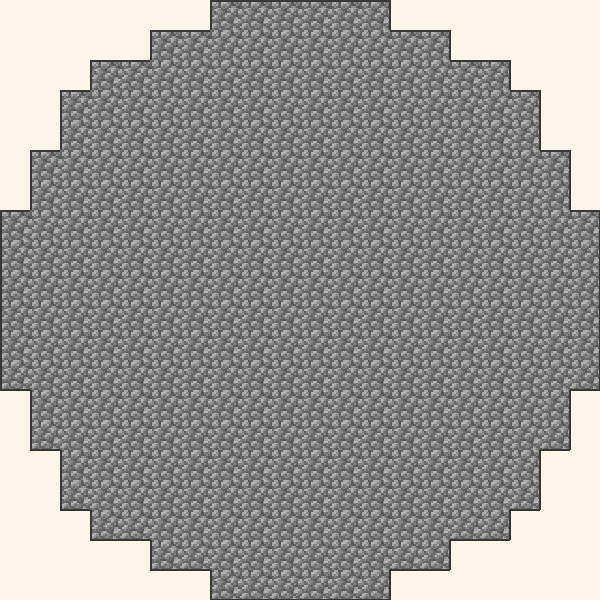
\includegraphics[width=\linewidth]{fig04_2d_d20_euclidean.png}
  \caption{\emph{Euclidean}}
\end{subfigure}\hfill
\begin{subfigure}[t]{0.31\linewidth}\centering
  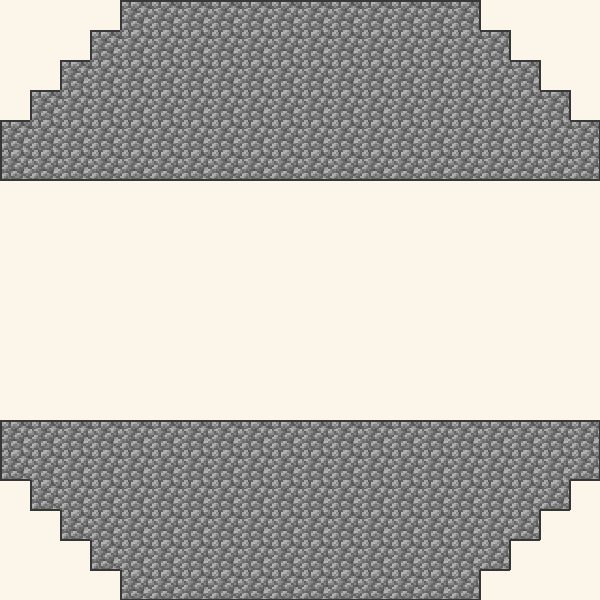
\includegraphics[width=\linewidth]{fig05_2d_d20_bresenham.png}
  \caption{\emph{Bresenham}}
\end{subfigure}\hfill
\begin{subfigure}[t]{0.31\linewidth}\centering
  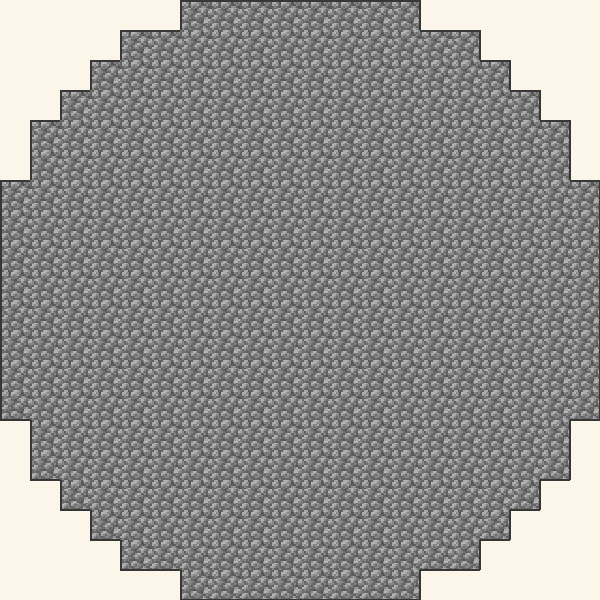
\includegraphics[width=\linewidth]{fig06_2d_d20_threshold.png}
  \caption{\emph{Threshold}}
\end{subfigure}
\caption{The same diameter-20 circle in the three algorithms, rendered in cobblestone texture. The larger diameter makes the differences more subtle --- to the naked eye, the three look similar. This is a good moment to note that for small diameters (Figure~\ref{fig:comp-d10}) the differences are far more evident.}
\label{fig:comp-d20}
\end{figure}

\begin{minecraft}[Block comparison: Block Round \emph{vs.} WorldEdit]
Try at home (if you have Minecraft + WorldEdit): run \cmd{//sphere stone 10} on a server and count the blocks. Compare with what Block Round reports in the \emph{Info chip} for the Bresenham algorithm, $D = 20$. The two counts should match (\emph{or} differ by 0--4 blocks due to small implementation differences). If you find a consistent difference, you have discovered a genuine mathematical curiosity.
\end{minecraft}

% =============================================================================
\subsection{Lesson 3 --- \enquote{From ellipse to ellipsoid: the third dimension}}\label{lesson3}

\subsubsection*{Lesson objective}
Generalize the equation of the ellipse to the ellipsoid, introduce voxels, discrete volume calculation, and planar cuts. Build bridges with American visual heritage and with notable constructions of the international Minecraft community.

\begin{activity}[3.1 --- From 2D to 3D equations \quad\timetag{15 min}]\label{at:31}
Add a third coordinate $z$ to the Cartesian plane. The implicit equation of the ellipse generalizes naturally:

\begin{formula}
\centering
$\displaystyle \left(\dfrac{x}{r_x}\right)^{\!2} + \left(\dfrac{y}{r_y}\right)^{\!2} + \left(\dfrac{z}{r_z}\right)^{\!2} \;=\; 1$
\end{formula}

When $r_x = r_y = r_z = r$, we recover the \acc{sphere} $x^2 + y^2 + z^2 = r^2$, as illustrated in Figure~\ref{fig:3d-shapes}.

\textbf{Voxels:} a cell of a 3D grid is called a \emph{voxel} (\emph{volume element}). In Minecraft, each voxel corresponds to a $1\times1\times1$ \emph{block}. The membership criterion is exactly the same as in 2D, with the added $z$ coordinate:

\begin{formula}
\centering
$\displaystyle a_x^2 + a_y^2 + a_z^2 \leq 1,\quad \text{with } a_\xi = \dfrac{\xi + \tfrac{1}{2} - c_\xi}{r_\xi}$
\end{formula}

\textbf{Demonstration:} open Block Round in 3D mode, switch between Sphere and Ellipsoid, rotate with the \emph{mouse}, observe the voxel structure.
\end{activity}

\begin{figure}[!htbp]
\centering
\begin{subfigure}[t]{0.45\linewidth}\centering
  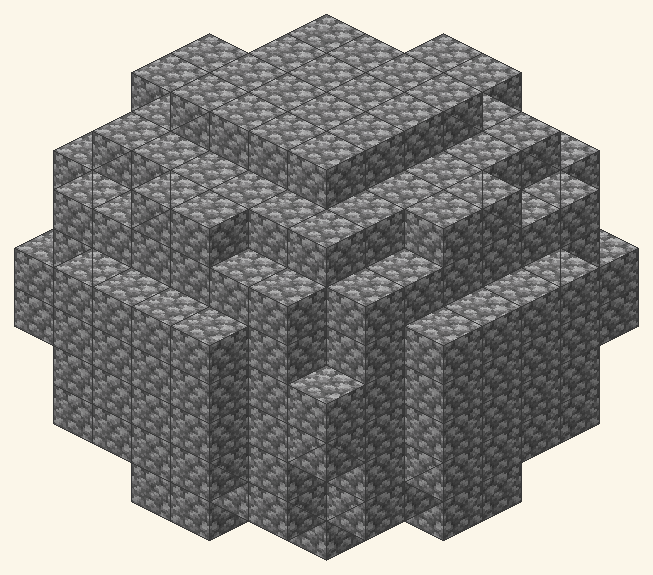
\includegraphics[width=\linewidth]{fig10_3d_sphere_d12.png}
  \caption{Diameter-10 sphere ($r_x = r_y = r_z = 5$).}
\end{subfigure}\hfill
\begin{subfigure}[t]{0.45\linewidth}\centering
  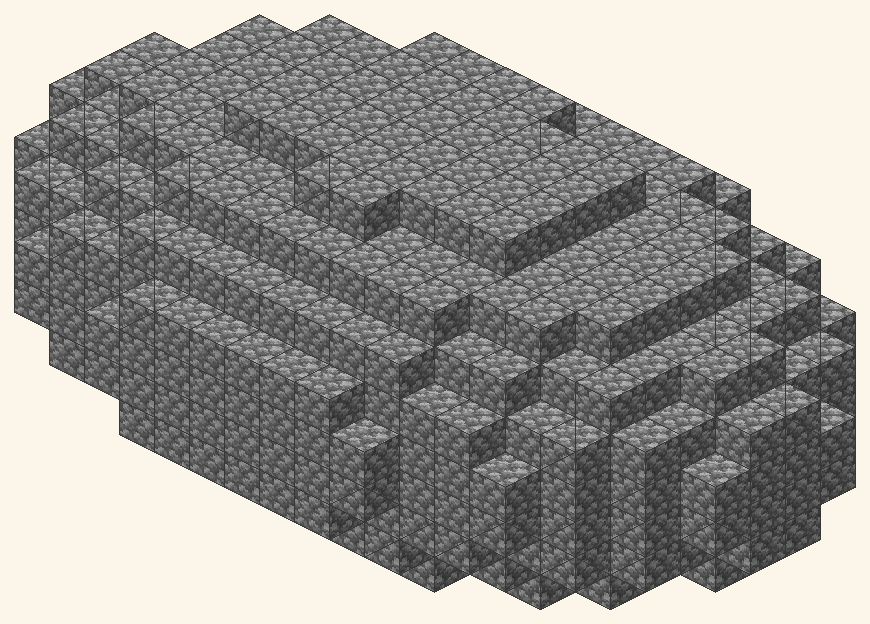
\includegraphics[width=\linewidth]{fig11_3d_ellipsoid.png}
  \caption{Ellipsoid with $W = 20, H = 10, D = 12$.}
\end{subfigure}
\caption{3D voxelization. Each cube is a voxel (= a Minecraft block); its $(i, j, k)$ center coordinate is tested in the implicit equation. The staircase patterns visible on the surface are characteristic of voxelization --- exactly the look that gives Minecraft its visual identity.}
\label{fig:3d-shapes}
\end{figure}

\begin{activity}[3.2 --- Continuous \emph{vs.} discrete volume \quad\timetag{15 min}]\label{at:32}
The continuous volume of the ellipsoid is a classical result:

\begin{formula}
\centering
$\displaystyle V \;=\; \dfrac{4}{3}\,\pi\, r_x\, r_y\, r_z$
\end{formula}

When $r_x = r_y = r_z = r$, $V = \tfrac{4}{3}\pi r^3$. This is content \acc{recurrent on the SAT, ACT, and AP exams} (questions on Solid Geometry appear on essentially every administration) and is also developed conceptually in AP Calculus AB/BC through the disk and shell methods for volumes of solids of revolution.

\textbf{Pair activity:}
\begin{enumerate}[leftmargin=1.5em,itemsep=0.15em,topsep=0.3em,nosep]
  \item Compute the continuous volume of a sphere with diameter 12 ($r = 6$): $V = \tfrac{4}{3}\pi \cdot 216 \approx 904.78$.
  \item In Block Round, generate the sphere $D = 12$, mode \emph{Filled}, activate \emph{Info chip}, record the discrete volume (number of blocks): approximately $V_{\mathrm{disc}} \approx 904$ blocks. \emph{Relative error $\approx 0.1\%$ --- remarkable.}
  \item In the same chip, observe the notation \emph{$904 = 14 \times 64 + 8$}: the game will tell a survival builder \enquote{you need \emph{14 full stacks} of cobblestone + one partial stack with \emph{8 blocks}}.
  \item Repeat for $D = 16$ ($V_{\mathrm{cont}} \approx 2{,}144$; $V_{\mathrm{disc}} \approx 2{,}145$). Note that for even $D$ the error can even be \emph{positive} (overestimation due to the center falling between cells).
\end{enumerate}

\textbf{Observation:} the ratio $\text{discrete volume}/\text{continuous volume} \to 1$ as $D \to \infty$. For small $D$, there is noticeable divergence --- and this is mathematically correct: discretization \emph{actually} alters the count.
\end{activity}

\begin{activity}[3.3 --- Planar cuts \quad\timetag{10 min}]\label{at:33}
Block Round allows cutting the ellipsoid by three different planes. Each cut is a \acc{linear inequality} applied to the voxel center:

\begin{formula}
\centering
$\begin{array}{lcl}
\text{X-axis:} & x \geq \mathit{cut} & \Rightarrow \text{voxel discarded} \\
\text{Y-axis:} & y \geq \mathit{cut} & \Rightarrow \text{voxel discarded} \\
\text{Diagonal:} & x + y \geq \mathit{cut} & \Rightarrow \text{voxel discarded}
\end{array}$
\end{formula}

Figure~\ref{fig:cortes} illustrates the three cuts at $50\%$.

\textbf{Directed discussion:} \emph{\enquote{Why does a diagonal cut have amplitude $D_x + D_y$ and not $D_x$? Where is the hypotenuse?}} Guide students to recognize that $x + y$ takes values between $0$ and $D_x + D_y$ in the bounding box. \emph{In Minecraft, a Y 50\% cut on a sphere produces the classic \enquote{dome} --- the upper half of the sphere, which is exactly the construction that covers temples, observatories, and arenas on thousands of servers.}
\end{activity}

\begin{figure}[!htbp]
\centering
\begin{subfigure}[t]{0.31\linewidth}\centering
  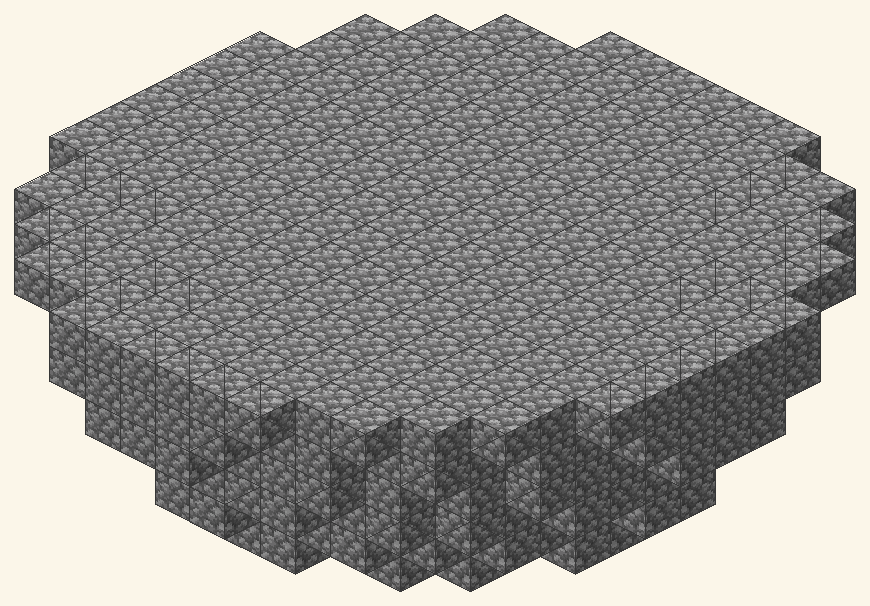
\includegraphics[width=\linewidth]{fig12_3d_cut_y50.png}
  \caption{Y cut at 50\% --- the classic \emph{dome}.}
\end{subfigure}\hfill
\begin{subfigure}[t]{0.31\linewidth}\centering
  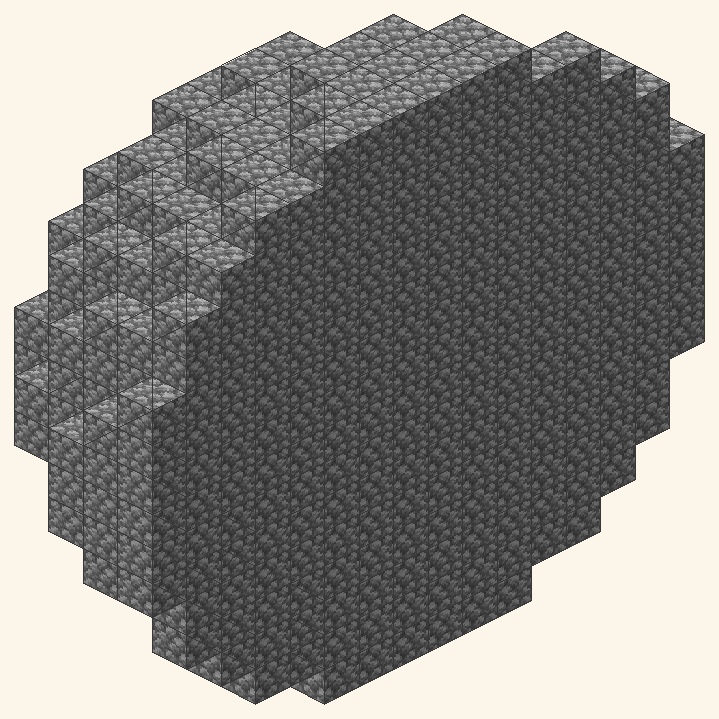
\includegraphics[width=\linewidth]{fig13_3d_cut_x50.png}
  \caption{X cut at 50\% --- a \emph{lateral half-sphere}.}
\end{subfigure}\hfill
\begin{subfigure}[t]{0.31\linewidth}\centering
  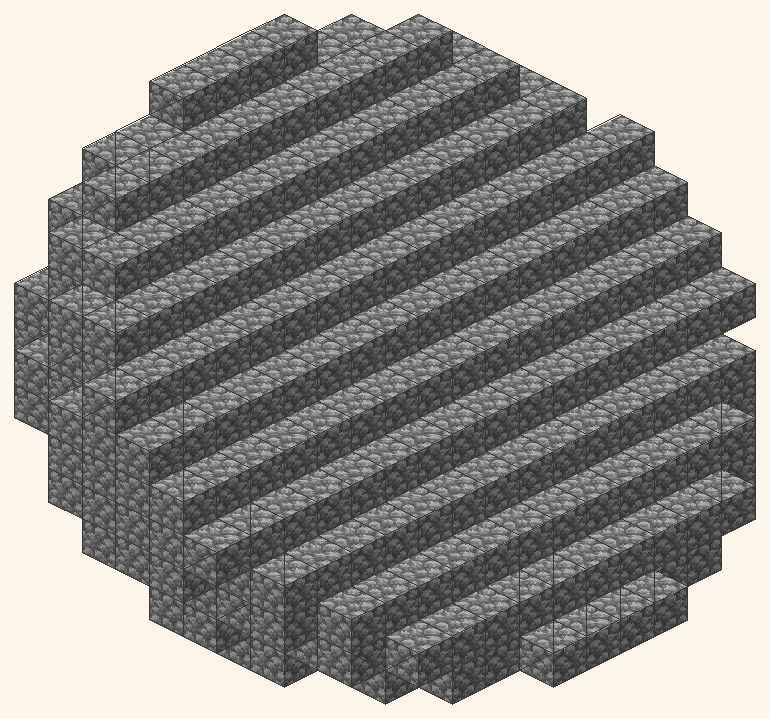
\includegraphics[width=\linewidth]{fig14_3d_cut_diag50.png}
  \caption{Diagonal cut at 50\% --- an \emph{oblique half-bowl}.}
\end{subfigure}
\caption{Three planar cuts on the same diameter-16 ellipsoid, each preserving $50\%$ of the volume. Note the characteristic stair-stepped pattern of the diagonal cut: it exposes the hypotenuse connecting the two axes. Each cut is a different Minecraft construction plan: temple dome, lateral half-arena, oblique amphitheater fountain.}
\label{fig:cortes}
\end{figure}

\begin{activity}[3.4 --- Dialogue with American visual heritage \quad\timetag{10 min}]\label{at:34}
\emph{Connection to Arts and History. This activity engages the cultural-identity and heritage standards in many state frameworks.}

Project (or hand out as printouts) five images:

\begin{itemize}[leftmargin=1.3em,itemsep=0.2em,topsep=0.3em,nosep]
  \item \acc{Frank Lloyd Wright's Solomon R. Guggenheim Museum} (New York, 1959) and \acc{Eero Saarinen's Gateway Arch} (St.\ Louis, 1965 --- a catenary curve, the surprise twin of the parabola): two American modernist landmarks where pure mathematical curves become architecture. Saarinen's TWA Flight Center at JFK (1962), with its elliptical wings, is openly elliptical in plan. The architectural moves of these designers mirror, at the scale of buildings, the quadric surfaces we are studying. (See Figure~\ref{fig:3d-shapes}(b) for an ellipsoidal volume.)

  \item \acc{Buckminster Fuller's geodesic dome} (Montreal Biosphère / U.S.\ Pavilion 1967 World's Fair; Spaceship Earth at Epcot in Walt Disney World): Fuller realized \emph{sphere tessellation} (geodesic subdivision) at architectural scale --- a direct mathematical connection to voxelization: like our discrete sphere, the geodesic dome approximates a smooth sphere using a finite number of flat panels. Fuller's wider \emph{Dymaxion} project (Dymaxion car, Dymaxion map) belongs to the same mathematical-aesthetic family.

  \item \acc{Pueblo kivas, Plains tipi, Navajo hogan, Wampanoag wetu, Anishinaabe wigwam}: the traditional dwellings of Indigenous peoples of North America often have circular, conic, or hemispherical floor plans. These architectural knowledges, transmitted orally across centuries, contain sophisticated geometry --- \emph{voxelization avant la lettre}. Contemporary continuation: the National Museum of the American Indian (NMAI, Washington DC, opened 2004) by Douglas Cardinal --- curvilinear stone whose façade has a voxel-like quality.

  \item \acc{Pueblo pottery and Navajo weaving} (Acoma, Zuni, Mata Ortiz lineage; diamond and stepped-diamond patterns): geometric traditions with documented spatial sophistication --- \emph{folded symmetries}, partition of space into circular and square zones. Tradition still vibrantly alive (Acoma potters, Hopi katsina drawings, Tlingit formline art, Anishinaabe Woodland Style). \emph{The stepped diamond is a direct voxel-style ancestor in textile.}

  \item \acc{Mound Builder geometry --- Cahokia Mounds} (Mississippian, Illinois --- UNESCO World Heritage Site), \acc{Hopewell mound complex} (Ohio), \acc{Serpent Mound} (Ohio), \acc{Pueblo of Mesa Verde} (Colorado, UNESCO): ceremonial earthworks featuring circles, ellipses, and precise alignment with celestial bodies. Pre-contact mathematical and astronomical sophistication, recognized internationally.

  \item \acc{International Minecraft community builds}: cities built on servers like Hermitcraft, MCC Island, Hypixel, or on school servers. Show timelapses of dome, sphere, and arch constructions published by creators like Pixlriffs, ilmango, Mumbo Jumbo, Grian, Etho, Pearlescent Moon. \emph{This is the contemporary, living ethnomathematics of Minecraft in action}, in English.
\end{itemize}

\textbf{Directed discussion:} \emph{\enquote{Fuller and Saarinen designed in steel and concrete the same curves you drew in blocks. Pueblo and Anishinaabe artisans represented circles and symmetries using pottery and weaving --- centuries before computers existed. The Mound Builders inscribed entire geometric ceremonial complexes in the earth a millennium ago. The Minecraft community does this live, every day, on shared servers. The rasterization problem we are studying is not an invention of the digital era: it is a constant of human history. Every culture has found its own way to \emph{rasterize}.}}

\textbf{Interdisciplinary connection:} suggested partnership with the Art teacher, History/Social Studies teacher, and/or Geography teacher for deepening. Lesson~\ref{lesson4} and Lesson~\ref{lesson5} may invite groups to \emph{choose} which visual tradition will inspire their work.

\textbf{Articulation with Minimalist and computational art:} the geometric grids of \emph{Frank Stella}, \emph{Sol LeWitt}, \emph{Donald Judd}, and \emph{Chuck Close} (gridded portraits --- direct pixel-art ancestors), along with the algorithmic art of \emph{Vera Molnar} and \emph{Manfred Mohr}, position voxel art within a clear lineage in modern and contemporary art collected by MoMA, the Whitney, the Met, and the National Gallery.
\end{activity}

% =============================================================================
\subsection{Lesson 4 --- \enquote{Inventory arithmetic: stacks, chests, commands}}\label{lesson4}

\subsubsection*{Lesson objective}
Introduce Minecraft \emph{inventory arithmetic} as a concrete application of ceiling division and quotient/remainder representation. Present the central commands (\cmd{/fill}, \cmd{/clone}, \cmd{//sphere}, \cmd{//hsphere}) and the octahedral-symmetry optimization.

\begin{activity}[4.1 --- Stack arithmetic \quad\timetag{15 min}]\label{at:41}
In Minecraft, each inventory slot holds at most \acc{64 identical blocks}. This limit is what gives practical meaning to volume calculation: $V = 904$ blocks for a $D=12$ sphere does \emph{not} mean \enquote{$904$ in the bag} --- it means \enquote{$\lceil 904/64 \rceil = 15$ \emph{stacks} (filled slots)} of cobblestone.

\textbf{Key formulas:}

\begin{formula}
\centering
$\displaystyle N_{\mathrm{stacks}} = \left\lceil \dfrac{V}{64} \right\rceil
\qquad\qquad
N_{\mathrm{double\,chests}} = \left\lceil \dfrac{V}{3{,}456} \right\rceil$
\end{formula}

(A single chest has 27 slots; a double chest, 54 slots; $54 \times 64 = 3{,}456$ items per double chest.)

\textbf{Pair activity:}
\begin{enumerate}[leftmargin=1.5em,itemsep=0.15em,topsep=0.3em,nosep]
  \item For a sphere $D = 8$ (volume $\approx 268$ blocks): how many stacks? How many single chests? Answer: 5 stacks; 1 single chest (with 17 slots free).
  \item For a sphere $D = 16$ (volume $\approx 2{,}145$ blocks): how many stacks? How many double chests? Answer: 34 stacks; 1 double chest (with 20 stacks of room to spare --- enough room for another small cylinder).
  \item For a sphere $D = 32$ (volume $\approx 17{,}156$ blocks): how many stacks? How many double chests? Answer: 269 stacks ($\approx 5$ double chests $+$ 1 stack), $\lceil 17{,}156/3{,}456 \rceil = 5$ double chests.
  \item \emph{In Minecraft survival mode, players typically mine 1 stack of cobblestone every 4--6 minutes (depending on the pickaxe). Compute total estimated collection time for the $D = 16$ sphere: $34 \times 5 = 170$ minutes $\approx 2.8$ hours.}
\end{enumerate}
\end{activity}

\begin{activity}[4.2 --- Minecraft commands \quad\timetag{15 min}]\label{at:42}
Introduce the central commands:

\begin{itemize}[leftmargin=1.4em,itemsep=0.25em,topsep=0.3em]
  \item \cmd{/setblock x y z minecraft:stone} --- places one block at a specific position.
  \item \cmd{/fill x1 y1 z1 x2 y2 z2 minecraft:stone} --- fills a rectangular box with a block. Vanilla limit: $32{,}768$ blocks per command.
  \item \cmd{/clone x1 y1 z1 x2 y2 z2 x3 y3 z3} --- copies a region to another position (fundamental power for symmetric construction).
  \item \cmd{//sphere stone 8} (WorldEdit) --- draws a radius-8 sphere centered on the player, using Bresenham 3D.
  \item \cmd{//hsphere stone 8} (WorldEdit) --- draws a \emph{hollow} sphere (shell only). Useful for hollow domes.
  \item \cmd{//ellipsoid stone 10 5 10} (WorldEdit) --- ellipsoid $W = 20, H = 10, D = 20$ with given semi-axes.
\end{itemize}

\textbf{Demonstration (if Minecraft is available):} run \cmd{//sphere stone 8} in a test world and time it. Compare with what Block Round shows for diameter 16, Bresenham algorithm. Confirm the mathematical identity of the two outputs.

\textbf{If Minecraft is not available:} run it mentally. Record on graph paper: \enquote{I'm on the ground (y=64). I want a radius-8 sphere starting at y=72 (8 blocks above the ground). What command?} Answer: \cmd{//sphere stone 8} while standing at $(0, 72, 0)$.
\end{activity}

\begin{activity}[4.3 --- Octahedral-symmetry optimization \quad\timetag{15 min}]\label{at:43}
\textbf{Central idea:} a sphere centered at the origin is invariant under reflections across the three coordinate planes. The group $\mathbb{Z}_2^3$ has order 8: starting from one \emph{octant} (region $+x, +y, +z$), the other seven regions are obtained by reflection.

\textbf{Practical implication:} instead of placing $V$ blocks one by one, build $V/8$ blocks in the positive octant and reflect 7 times with \cmd{/clone}.

\begin{formula}
\centering
$\displaystyle \mathrm{cost}_\mathrm{symmetry} = N_\mathrm{octant} + 7\, T_\mathrm{clone}
\;\ll\; \mathrm{cost}_\mathrm{bruteforce} = N\, T_\mathrm{block}$
\end{formula}

\textbf{Concrete example, sphere $D = 24$ centered at $(0, 72, 0)$:}
\begin{enumerate}[leftmargin=1.5em,itemsep=0.15em,topsep=0.3em,nosep]
  \item Manually build the positive octant ($\approx 905$ blocks, $\approx 15$ minutes in survival or $\approx 45$ seconds in creative with brush).
  \item Reflect to $-x$: \cmd{/clone 0 72 0 12 84 12 -12 72 0 mode:masked}
  \item Reflect to $-y$: \cmd{/clone 0 72 0 12 84 12 0 60 0 mode:masked}
  \item Reflect to $-z$: \cmd{/clone 0 72 0 12 84 12 0 72 -12 mode:masked}
  \item Octants $(-x, -y)$, $(-y, -z)$, $(-x, -z)$, $(-x, -y, -z)$: analogous commands.
\end{enumerate}

\textbf{Time comparison:}
\begin{itemize}[leftmargin=1.3em,itemsep=0.1em,topsep=0.2em,nosep]
  \item Without symmetry, in survival: $7{,}238$ blocks $\times$ 2 s/block $\approx$ 4 hours.
  \item With symmetry: 15 min (octant) + 0.5 s (7 clones) $\approx$ 15 min.
  \item Speedup: \emph{factor of 16}.
\end{itemize}
\end{activity}

\begin{activity}[4.4 --- Application: planning a real dome \quad\timetag{5 min}]
In pairs, plan (\emph{on paper or in Block Round}) the construction of a Quartz dome $D=20$ atop a stylized temple (Pueblo-, Saarinen-, or Fuller-inspired). Record:
\begin{itemize}[leftmargin=1.3em,itemsep=0.1em,topsep=0.2em,nosep]
  \item Volume of the dome (half-sphere $D=20$): $\approx 2{,}094$ blocks.
  \item Stacks required: 33 stacks.
  \item Number of Quartz blocks (each requires 4 Nether Quartz, mined in the Nether): $\sim 2{,}094 \times 4 = 8{,}376$ Nether Quartz.
  \item Optimized command sequence using symmetry.
\end{itemize}

This activity sets the stage for Lesson 5 (real construction).
\end{activity}

% =============================================================================
\subsection{Lesson 5 --- \enquote{Real construction: from Block Round to Minecraft}}\label{lesson5}

\subsubsection*{Lesson objective}
Mobilize all developed content in an \emph{authorial built product}: export from Block Round, import into Minecraft (via Litematica or Schematica), execute the construction in creative or survival. Assess learning through argumentative defense of mathematical choices and delivery of the final product.

\begin{activity}[5.1 --- Challenge presentation \quad\timetag{5 min}]\label{at:51}
\textbf{Instruction:} \emph{\enquote{In pairs or trios, you will produce a Minecraft construction (or, if Minecraft is unavailable, in Block Round) that combines at least three figures generated by Block Round (circles, ellipses, spheres, or ellipsoids). It can be a city on the class server, a temple, a round farm, an observatory --- you choose. At the end, each group will present the work explaining \acc{mathematically} the choices: why this algorithm? why this proportion? why this cut? why these blocks?}}
\end{activity}

\begin{activity}[5.2 --- Export and import \quad\timetag{15 min}]\label{at:52}
Demonstrate the Block Round $\rightarrow$ Minecraft flow:

\begin{enumerate}[leftmargin=1.5em,itemsep=0.2em,topsep=0.3em]
  \item In Block Round, configure the desired figure (e.g.\ Quartz $D = 12$ sphere with Y 50\% cut).
  \item Click the \emph{Export Schematic} button at the corner of the canvas. The \texttt{.schem} file (Sponge Schematic v2) is downloaded.
  \item In Minecraft Java Edition with the \emph{Litematica} mod installed (free): open the mod, \emph{Load Schematic}, select the downloaded file.
  \item Litematica shows a translucent \enquote{ghost} of the construction at the position the player chooses.
  \item The player places each block \emph{following the ghost}. Litematica highlights any out-of-place block in red.
  \item \emph{Alternative via \cmd{//schem load}:} on a server with WorldEdit, \cmd{//schem load filename} imports the schematic, and \cmd{//paste -a} pastes at the current position --- instant construction.
\end{enumerate}

\textbf{If Minecraft is not available:} demonstrate \texttt{.schem} export and view the binary file with a hex editor --- discussion of Sponge v2 format, gzip, NBT. CTE Information Technology articulation.
\end{activity}

\begin{activity}[5.3 --- Production \quad\timetag{20 min}]\label{at:53}
\textbf{Group materials:}
\begin{itemize}[leftmargin=1.3em,itemsep=0.15em,topsep=0.3em,nosep]
  \item Access to Block Round (computer or \emph{smartphone});
  \item (Optional) Access to Minecraft with Litematica or Schematica;
  \item Graph paper, pencil, and colored pencils for sketches and outlines;
  \item Worksheet with three required questions (Appendix~\ref{ap:exerc}, exercise 8).
\end{itemize}

\textbf{Internal group-work stages:}
\begin{enumerate}[leftmargin=1.5em,itemsep=0.15em,topsep=0.3em,nosep]
  \item \timetag{5 min} Brainstorm and paper sketch.
  \item \timetag{8 min} Production in Block Round and \texttt{.schem} export.
  \item \timetag{5 min} Import into Minecraft and quick test (if available).
  \item \timetag{2 min} Write up the mathematical justification on the worksheet.
\end{enumerate}

\textbf{Teacher support:} circulate among groups, asking mediating questions --- \emph{\enquote{Why did you choose that algorithm? How could this cut be described as an inequality? How many double chests of Quartz will you need?}}
\end{activity}

\begin{activity}[5.4 --- Presentation and collective synthesis \quad\timetag{10 min}]\label{at:54}
Each group has 2 minutes to present the work to the class, showing it on the projector (or in Minecraft, or physically on paper), and answering \emph{at least one} of the three required mathematical questions.

\textbf{Minimum presentation criteria:}
\begin{itemize}[leftmargin=1.3em,itemsep=0.1em,topsep=0.2em,nosep]
  \item identify at least one mathematical figure present;
  \item name the chosen algorithm and justify (even \emph{a posteriori}) why it fits the intended visual effect;
  \item if there is a 3D cut, describe it as an inequality;
  \item estimate (even roughly) the number of stacks/chests required.
\end{itemize}

\textbf{Teacher's final synthesis (3 min):} return to the central idea of the sequence --- \emph{\enquote{on a discrete voxel grid, the same continuous curve admits multiple representations; choosing one is making a mathematical decision; building it in Minecraft is making a decision of citizenship, resource management, and aesthetics}} --- and situate it on the horizon of contemporary American mathematics: invite the class to explore the \hyperref[sec:olympiad]{AMC 10/12} and AIME, to learn more about Maryam Mirzakhani, Terence Tao, June Huh, and other Fields medalists who worked or trained in the U.S., and to participate in Minecraft servers that promote collaborative construction.
\end{activity}

\begin{minecraft}[Extension possibilities]
This Lesson 5 opens up several extension possibilities in extracurricular projects:
\begin{itemize}[leftmargin=1.3em,itemsep=0.15em,topsep=0.3em,nosep]
  \item \textbf{Math City Project:} the class builds a city on the school server, where each building implements a geometric figure (cylinder, sphere, ellipsoid, set of conics).
  \item \textbf{American heritage recreation:} Minecraft reconstruction of the Gateway Arch (St.\ Louis), the Guggenheim NYC, Spaceship Earth at Epcot, Walt Disney Concert Hall (Los Angeles), Cahokia Mounds, or a Pueblo Bonito (Chaco Canyon).
  \item \textbf{Block Round Olympiad:} internal competition --- who builds the sphere closest to the continuous volume? who optimizes time best via symmetry?
  \item \textbf{Engineering articulation (CTE / PLTW):} use Block Round as a pre-engineering sandbox: geodesic domes, voxelized trusses, structures approximating smooth surfaces. Direct integration with Project Lead The Way (PLTW) Engineering and Engineering Design curricula.
  \item \textbf{Programming articulation (AP CSP, USACO):} re-implement the three algorithms in Python or JavaScript, compare outputs with Block Round, submit the analysis as a science-fair project or USACO competition entry.
\end{itemize}
\end{minecraft}

% =============================================================================
\section{Assessment}\label{sec:assessment}

Assessment adopts a \acc{formative}, \acc{processual}, and \acc{summative} model, articulating four dimensions (plus a specific dimension for the Minecraft application) and dialoguing with the U.S. tradition of standards-based grading and the practices of formative assessment described by Wiliam (\emph{Embedded Formative Assessment}, 2011) and Marzano (\emph{Classroom Assessment and Grading That Work}, 2006).

\subsection{Diagnostic assessment}
Conducted in Lesson~\ref{lesson1}, at the moment of Activity 1.2 (hand-drawing of the circle). Allows the teacher to identify difficulties with the Cartesian plane, equation of the circle, and counting --- and to address post-pandemic gaps evidenced by the 2022 NAEP results.

\subsection{Formative assessment}
Distributed across the five lessons: direct observation of participation, quality of responses in the \emph{think--pair--share}, \emph{immediate} correction of calculations in Activities~\ref{at:25}, \ref{at:32}, and~\ref{at:41}.

\subsection{Summative assessment}
Composed of two deliverables:

\begin{enumerate}[leftmargin=1.5em,itemsep=0.2em,topsep=0.3em,nosep]
  \item \textbf{Problem set} (Appendix~\ref{ap:exerc}), 8 questions, due at the end of Lesson~\ref{lesson5} or on an agreed date.
  \item \textbf{Final project} (Activity~\ref{at:53}), with the worksheet completed during the defense (Activity~\ref{at:54}).
\end{enumerate}

\subsection{Assessment rubric}

\begin{center}
\small
\begin{tabularx}{\textwidth}{@{}p{0.21\textwidth}XX@{}}
\toprule
\textbf{Dimension} & \textbf{Fully proficient (8--10)} & \textbf{Partially proficient (5--7) / Insufficient (0--4)} \\
\midrule
\textbf{Mathematical concepts} & Correctly applies the implicit equation of the ellipse/ellipsoid; recognizes the three algorithmic criteria and their differences. & Applies the basic equation of the circle but gets confused with the generalization to the ellipse / does not distinguish the algorithms. \\
\addlinespace[3pt]
\textbf{Software use (Block Round)} & Operates Block Round autonomously in 2D and 3D; exports images and \texttt{.schem}; toggles algorithms and styles. & Needs frequent assistance; operates 2D only. \\
\addlinespace[3pt]
\textbf{Argumentation} & Justifies project choices mathematically; uses appropriate technical vocabulary (\emph{algorithm}, \emph{voxel}, \emph{cut}, \emph{inequality}, \emph{stack}, \emph{double chest}). & Justifies aesthetically without mobilizing mathematics; vocabulary absent. \\
\addlinespace[3pt]
\textbf{Practical Minecraft application} & Correctly computes stacks and chests for the project; describes a \cmd{/fill} or \cmd{//sphere} command sequence; uses octahedral symmetry. & Confuses quotient and remainder; treats blocks as loose units; does not use symmetry. \\
\addlinespace[3pt]
\textbf{Cooperation} & Works productively in pair/trio; contributes to the collective discussion. & Works in isolation; minimal contribution. \\
\bottomrule
\end{tabularx}
\end{center}

\subsection{Grade conversion}
\begin{itemize}[leftmargin=1.3em,itemsep=0.1em,topsep=0.2em,nosep]
  \item Problem set: 40\% of grade.
  \item Final project + presentation: 50\% of grade.
  \item Process observation (participation): 10\% of grade.
\end{itemize}

% =============================================================================
\section{Articulations with the American mathematics ecosystem}\label{sec:olympiad}

The sequence is embedded in a \emph{rich ecosystem} of American initiatives in mathematics and technology education and research, which the teacher can mobilize for extension or deepening.

\subsection{AMC 10/12 --- American Mathematics Competitions}

Organized by the \acc{MAA} (Mathematical Association of America), the \href{https://www.maa.org/math-competitions}{AMC 10/12} and the subsequent AIME (American Invitational Mathematics Examination) and USAMO (USA Math Olympiad) form the official competition ladder leading to the U.S. team for the International Mathematical Olympiad (IMO). Hundreds of thousands of U.S. students sit the AMC every year, including from many public high schools (often via the math club).

\emph{The content of this sequence (analytic geometry of the circle and ellipsoid, algorithmic reasoning, numerical approximations) is directly preparatory for AMC 10/12 questions on geometry, counting, and computational thinking.}

\subsection{Summer programs and undergraduate research}

Top high school students can apply to nationally recognized summer programs that extend mathematics learning beyond the school year: \acc{MIT PRIMES} (research with MIT faculty), \acc{Stanford SUMaC} (Stanford University Mathematics Camp), \acc{RSI} (Research Science Institute, MIT), \acc{MathILy}, \acc{AwesomeMath}, \acc{Canada/USA Mathcamp}, and the \acc{Ross Mathematics Program} (Ohio State). This sequence's final project can serve as an entry portfolio piece. Additionally, the \emph{Park City Mathematics Institute (PCMI)} and the \emph{Math for America (MfA)} fellowships support teachers in this ecosystem.

\subsection{Fields medalists and U.S. mathematics}

The \emph{Fields Medal} is the most prestigious recognition in mathematics. Several Fields medalists worked or trained in the U.S. and are role models for students:

\begin{itemize}[leftmargin=1.3em,itemsep=0.15em,topsep=0.3em]
  \item \acc{Maryam Mirzakhani} (Stanford, Fields 2014) --- the \emph{first woman ever} to receive the Fields Medal. Worked on Riemann surfaces, hyperbolic geometry, and dynamics. Her story is essential pedagogy for representation in mathematics.
  \item \acc{Terence Tao} (UCLA, Fields 2006) --- known to a generation of students through his blog and YouTube. A model of public mathematician.
  \item \acc{June Huh} (Princeton, Fields 2022) --- exceptional story: started as a poetry student, found his way to math late. A counter to the myth that talent must show early.
  \item \acc{Edward Witten} (Institute for Advanced Study, Fields 1990) --- the first physicist to win the Fields Medal; bridges between mathematics and theoretical physics.
  \item \acc{William Thurston} (Fields 1982), \acc{Charles Fefferman} (Princeton, Fields 1978), \acc{Stephen Smale} (Fields 1966), \acc{John Milnor} (Institute for Advanced Study, Fields 1962) --- foundational American mathematicians whose work shaped topology, analysis, and geometry.
\end{itemize}

The major American mathematics research centers --- the \href{https://www.ias.edu/}{Institute for Advanced Study} (Princeton), \href{https://www.slmath.org/}{Mathematical Sciences Research Institute (SLMath/MSRI, Berkeley)}, \href{https://www.aimath.org/}{American Institute of Mathematics (AIM)}, and the \href{https://www.claymath.org/}{Clay Mathematics Institute} --- host scholars working at the cutting edge.

\subsection{USACO --- USA Computing Olympiad}

The \href{http://usaco.org/}{USA Computing Olympiad (USACO)} runs four contests per year and selects the U.S. team for the International Olympiad in Informatics (IOI). Bresenham's algorithm and computational geometry are recurring themes in USACO's Bronze, Silver, Gold, and Platinum divisions (treated in Activity~\ref{at:23}).

\subsection{Minecraft Education Edition (Microsoft Education)}\label{sec:mee}

The \emph{Minecraft Education Edition} is an educational variant available free to licensed K--12 schools through Microsoft Education (M365 EDU subscriptions). It includes pedagogy-specific features (screen camera, photo export, \emph{Code Builder} mode for visual block programming). With over 35 million users globally, MEE is aligned with the ISTE Standards and many state computer science frameworks. \emph{This sequence is compatible}: the \texttt{.schem} exported by Block Round can be imported in Java Edition (via Litematica) and adapted for Education Edition (via cmdblocks or indirect import).

\subsection{American Minecraft creator community}

The English-language Minecraft community maintains active channels specialized in \emph{redstone engineering} (computational logic implemented through in-game circuits --- equivalent to real digital circuits, descended from George Boole and Claude Shannon's foundational work at Bell Labs) and in \emph{megabuild architecture}. Creators like \emph{Pixlriffs}, \emph{ilmango}, \emph{Mumbo Jumbo} (technically UK-based, with a massive U.S. audience), \emph{Grian}, \emph{Etho}, \emph{Pearlescent Moon}, and the entire \emph{Hermitcraft} season community, plus servers like \emph{MCC Island}, \emph{Hypixel}, and the \emph{Minecraft Championship}, are cultural references the teacher can leverage for context. \emph{Complementary activity:} ask students to bring a tutorial link and analyze the implicit mathematics within it.

\subsection{Ethnomathematics and multicultural mathematics education}

The line of research in Ethnomathematics, founded by Brazilian mathematician \acc{Ubiratan D'Ambrosio} (1932--2021) and developed in the U.S. by \acc{Marcia Ascher} (\emph{Ethnomathematics: A Multicultural View of Mathematical Ideas}, 1991), received the ICMI Felix Klein Award (2005). The work of \acc{Deborah Loewenberg Ball} (Michigan) on mathematical knowledge for teaching, and of \acc{Rochelle Gutiérrez} (Illinois) on rehumanizing mathematics, extend this tradition into U.S. mathematics education.

\subsection{Teacher development pathways}

For teacher development, the principal national fellowships are \href{https://www.mathforamerica.org/}{Math for America (MfA)} (initially New York City, now broader), the \href{https://knowles.org/}{Knowles Teaching Fellowship}, the \href{https://www.parkcitymath.org/}{Park City Mathematics Institute (PCMI)}, and the NSF-funded \emph{Robert Noyce Teacher Scholarship}. The \href{https://www.nctm.org/}{National Council of Teachers of Mathematics (NCTM)} provides the principal professional community for K--12 math teachers; its \emph{Mathematics Teacher: Learning and Teaching PK--12} journal is a key venue for sequences such as this.

% =============================================================================
\section{Interdisciplinary articulations}\label{sec:interdisc}

\subsection{With Art (Visual and Performing Arts)}
The production of \emph{voxel art} is traditionally treated as an artistic language. Block Round offers a rare opportunity to articulate Mathematics and Art under the same object: the figure \emph{is simultaneously} an equation and an aesthetic composition. Suggestion: partner with an Art teacher for a final exhibition of the works on the school's bulletin board or social media. Possible deepening: study of American Minimalist and conceptual artists --- Frank Stella (geometric grids), Sol LeWitt (combinatorial drawings), Donald Judd (modular sculpture), Chuck Close (gridded portraits --- direct pixel-art ancestor), Vera Molnar and Manfred Mohr (algorithmic art). These artists' works are in the permanent collections of MoMA (NYC), the Whitney, the Met, SFMoMA, the National Gallery of Art (Washington), and the Hirshhorn (DC).

\subsection{With Physics (Natural Sciences, NGSS)}
The Block Round audio layer (when active) uses additive synthesis of sinusoidal waves (similar to its sibling Pixel Round). The chosen frequencies approximate notes of the \acc{12-tone equal temperament} (each semitone multiplies frequency by $2^{1/12} \approx 1.0595$). Content articulated with \emph{Mechanical Waves}, \emph{Acoustics}, and \emph{Exponential Functions}. In Minecraft, articulation with \emph{redstone} (digital logic --- the same Boolean algebra of George Boole and the information-theoretic foundations of Claude Shannon at Bell Labs), \emph{note blocks} (musical notation in-game), and \emph{physics simulation} (sand falling, water flow).

\subsection{With Computer Science (CS pathways)}
Bresenham's algorithm is a classic reference in Computer Science. Articulate with \emph{computational thinking} lessons: \emph{abstraction} (the equation as model), \emph{decomposition} (the shape as set of voxels), \emph{pattern recognition} (symmetries), \emph{algorithm design} (the three procedures). Direct connection with \hyperref[sec:olympiad]{USACO}, AP Computer Science Principles, AP Computer Science A, and with the K--12 CSTA framework. The \texttt{.schem} generation (Sponge v2 format with gzip + NBT) is a \emph{case study} in binary serialization --- content for CTE Information Technology coursework and for Project Lead The Way (PLTW) Computer Science programs. Code.org's CS Principles curriculum and the \emph{Computer Science for All} initiative (launched by the Obama administration in 2016) provide curricular context.

\subsection{With History (Social Studies)}
Bresenham published the algorithm in 1965, during the peak of \emph{mainframe} computing at IBM. The same era saw a transformation of computing in the United States: \emph{ENIAC} at UPenn (1945--1946, first general-purpose electronic computer); the Mark I at Harvard (Howard Aiken, 1944); \emph{Whirlwind} at MIT (1951, pioneer of real-time computing); the work of Grace Hopper (Mark I, then COBOL), Mary Allen Wilkes (LINC, 1965), and Margaret Hamilton (Apollo Guidance Computer). Bell Labs (Shannon's information theory, the transistor) was the engine of much of this revolution. \emph{Minecraft was launched in 2009 by Markus \enquote{Notch} Persson (Sweden), sold to Microsoft in 2014 for \$2.5 billion, and surpassed 300 million copies sold by 2023, becoming the best-selling video game in history (surpassing Tetris).} The game's trajectory intersects with the popularization of the internet, of personal computing, and of educational technology in U.S. public schools since the 2010s, including the \emph{Computer Science for All} initiative (2016) and the COVID-19 emergency funding (ESSER, 2020--2024). C3 Framework (College, Career, and Civic Life) connections are direct.

\subsection{With Geography (Social Studies)}
Rasterization is not just a \emph{voxel art} topic: it is the basis of \emph{geographic information systems} (GIS). Digital maps, satellite imagery (the NASA Landsat program --- over 50 years of continuous Earth observation), USDA agricultural mapping, USGS digital elevation models, the National Hurricane Center's storm modeling, and Esri's ArcGIS (developed in Redlands, CA) are contemporary American examples of the same mathematical problem the sequence addresses. \emph{Minecraft Earth} (discontinued 2021) was an experiment in \emph{augmented reality} that overlaid the voxel universe on real city maps in the U.S. and worldwide.

\subsection{With Engineering (CTE and PLTW pathways)}
Minecraft is \emph{notably} used in CTE engineering programs and in PLTW (Project Lead The Way) Engineering curricula as a pre-engineering sandbox: students simulate cities, electrical systems via redstone, hydraulic systems with water, mechanical systems with pistons and observers. The voxelized geometry introduced in this sequence is \emph{mental math} for anyone going into \emph{Mechanical Engineering}, \emph{Strength of Materials}, or \emph{Structural Engineering} --- particularly the \emph{finite element analysis (FEA)} of meshing, where voxels (or tetrahedra) discretize a continuous body for numerical simulation. The Engineering is Elementary curriculum (Museum of Science, Boston) and the National Academy of Engineering's \emph{Grand Challenges} program provide additional articulation points.

% =============================================================================
\section{References}\label{sec:references}

\subsection{Pedagogy and Mathematics Education (U.S. and international)}
\begin{itemize}[leftmargin=1.3em,itemsep=0.15em,topsep=0.3em]
  \item ASCHER, M. \emph{Ethnomathematics: A Multicultural View of Mathematical Ideas}. Pacific Grove: Brooks/Cole, 1991.
  \item BALL, D. L.; THAMES, M. H.; PHELPS, G. Content Knowledge for Teaching: What Makes It Special? \emph{Journal of Teacher Education}, v.~59, n.~5, p.~389--407, 2008.
  \item BOALER, J. \emph{Mathematical Mindsets: Unleashing Students' Potential through Creative Math, Inspiring Messages, and Innovative Teaching}. San Francisco: Jossey-Bass, 2015.
  \item D'AMBROSIO, U. \emph{Ethnomathematics: Link Between Traditions and Modernity}. Rotterdam: Sense Publishers, 2006.
  \item DEWEY, J. \emph{Democracy and Education}. New York: Macmillan, 1916.
  \item DEWEY, J. \emph{Experience and Education}. New York: Macmillan, 1938.
  \item GUTIÉRREZ, R. The Sociopolitical Turn in Mathematics Education. \emph{Journal for Research in Mathematics Education}, v.~44, n.~1, p.~37--68, 2013.
  \item MARZANO, R. J. \emph{Classroom Assessment and Grading That Work}. Alexandria: ASCD, 2006.
  \item PAPERT, S. \emph{Mindstorms: Children, Computers, and Powerful Ideas}. New York: Basic Books, 1980.
  \item POLYA, G. \emph{How to Solve It}. Princeton: Princeton University Press, 1945.
  \item SCHOENFELD, A. H. \emph{Mathematical Problem Solving}. Orlando: Academic Press, 1985.
  \item VYGOTSKY, L. S. \emph{Mind in Society: The Development of Higher Psychological Processes}. Cambridge: Harvard University Press, 1978.
  \item WILIAM, D. \emph{Embedded Formative Assessment}. Bloomington: Solution Tree, 2011.
\end{itemize}

\subsection{Studies of games and Minecraft in education}
\begin{itemize}[leftmargin=1.3em,itemsep=0.15em,topsep=0.3em]
  \item GEE, J. P. \emph{What Video Games Have to Teach Us About Learning and Literacy}. New York: Palgrave Macmillan, 2003.
  \item PRENSKY, M. \emph{Digital Game-Based Learning}. St.\ Paul: Paragon House, 2007.
  \item SCHRIER, K. \emph{Knowledge Games: How Playing Games Can Solve Problems, Create Insight, and Make Change}. Baltimore: Johns Hopkins University Press, 2016.
  \item SQUIRE, K. \emph{Video Games and Learning: Teaching and Participatory Culture in the Digital Age}. New York: Teachers College Press, 2011.
  \item STEINKUEHLER, C.; SQUIRE, K.; BARAB, S. (eds.). \emph{Games, Learning, and Society: Learning and Meaning in the Digital Age}. Cambridge: Cambridge University Press, 2012.
  \item Microsoft. \emph{Minecraft Education Edition portal}. Available at \url{https://education.minecraft.net}.
\end{itemize}

\subsection{Official documents and frameworks}
\begin{itemize}[leftmargin=1.3em,itemsep=0.15em,topsep=0.3em]
  \item National Governors Association Center for Best Practices, Council of Chief State School Officers. \emph{Common Core State Standards for Mathematics}. Washington, DC: NGA Center and CCSSO, 2010.
  \item U.S. Department of Education. \emph{Every Student Succeeds Act (ESSA)}. 2015.
  \item College Board. \emph{AP Calculus AB and BC Course and Exam Description}. New York: College Board, 2020.
  \item College Board. \emph{AP Precalculus Course and Exam Description}. New York: College Board, 2023.
  \item ISTE. \emph{ISTE Standards for Students}. Eugene: ISTE, 2016.
  \item CSTA. \emph{K--12 Computer Science Standards}. Computer Science Teachers Association, 2017.
  \item National Council of Teachers of Mathematics (NCTM). \emph{Principles to Actions: Ensuring Mathematical Success for All}. Reston: NCTM, 2014.
  \item U.S. Department of Education. \href{https://studentprivacy.ed.gov/}{\emph{Family Educational Rights and Privacy Act (FERPA)}}, 20 U.S.C. §1232g, 1974.
  \item Federal Trade Commission. \emph{Children's Online Privacy Protection Rule (COPPA)}, 16 CFR Part 312, 1998.
\end{itemize}

\subsection{Technical references}
\begin{itemize}[leftmargin=1.3em,itemsep=0.15em,topsep=0.3em]
  \item BRESENHAM, J. E. Algorithm for computer control of a digital plotter. \emph{IBM Systems Journal}, v.~4, n.~1, p.~25--30, 1965.
  \item PITTEWAY, M. L. V. Algorithm for drawing ellipses or hyperbolae with a digital plotter. \emph{The Computer Journal}, v.~10, n.~3, p.~282--289, 1967.
  \item Sponge Schematic specification v2, available at \url{https://github.com/SpongePowered/Schematic-Specification}.
  \item WorldEdit documentation, \url{https://worldedit.enginehub.org}.
  \item Block Round --- technical document: \texttt{docs\_math/Block\_Round\_Math\_en-US.pdf}.
\end{itemize}

\subsection{Mathematics history and culture}
\begin{itemize}[leftmargin=1.3em,itemsep=0.15em,topsep=0.3em]
  \item BELLOS, A. \emph{Alex's Adventures in Numberland}. London: Bloomsbury, 2010.
  \item DEVLIN, K. \emph{The Math Gene: How Mathematical Thinking Evolved and Why Numbers Are Like Gossip}. New York: Basic Books, 2000.
  \item FRIES-GAITHER, J. \emph{Math Anywhere}. NSTA Kids, 2020.
  \item HUH, J. Interview. \emph{Quanta Magazine}, 2022.
  \item ISAACSON, W. \emph{The Innovators: How a Group of Hackers, Geniuses, and Geeks Created the Digital Revolution}. New York: Simon \& Schuster, 2014.
  \item LOCKHART, P. \emph{A Mathematician's Lament}. New York: Bellevue Literary Press, 2009.
  \item Mathematical Association of America (MAA). \emph{AMC 10/12 problem archives and AIME problems}. Available at \url{https://www.maa.org/math-competitions}.
\end{itemize}

\newpage
% =============================================================================
% APPENDICES
% =============================================================================
\appendix
\renewcommand{\thesection}{\Alph{section}}
\setcounter{section}{0}

\section{Block Round live demonstration script}\label{ap:roteiro}

Recommended sequence for the initial demonstration (Activity~1.3) and for teacher familiarization. Total time: 15 minutes.

\subsection{Opening and 2D mode}
\begin{enumerate}[leftmargin=1.5em,itemsep=0.15em,topsep=0.3em]
  \item Open Block Round (\url{https://vinisouza128.github.io/block-round/}). With the class, observe the visible elements: top bar, central drawing area (\emph{canvas}), side controls, block picker below.
  \item Confirm that the mode is on \acc{2D / Circle}.
  \item Adjust the \emph{Size} slider to 10. Observe the figure (compare with Figure~\ref{fig:comp-d10}(a) in this plan).
  \item In the lower corner of the canvas, activate the \emph{Info chip} button. The class should read aloud: \enquote{Diameter 10, Radius 5, Blocks $\dots$, Algorithm Euclidean}.
  \item Toggle between the three algorithms by clicking the \emph{pills} \acc{Euclidean} / \acc{Bresenham} / \acc{Threshold}. Pause on each for 30 seconds.
\end{enumerate}

\subsection{Block textures}

\begin{enumerate}[leftmargin=1.5em,itemsep=0.15em,topsep=0.3em]
  \item Keep the diameter at 10 and Euclidean algorithm.
  \item Demonstrate block swapping: click \emph{Cobblestone}, then \emph{Oak Planks}, then \emph{Quartz Block}, then \emph{Diamond}. Observe that the shape \emph{does not change} --- only the texture.
  \item Discussion: \emph{\enquote{You're seeing the same sphere --- the math is identical. Only the dress has changed. In Minecraft, you pick the block; here, you pick the texture to visualize.}}
\end{enumerate}

\needspace{18\baselineskip}
\subsection{Ellipse}

\begin{figure}[!htbp]
\centering
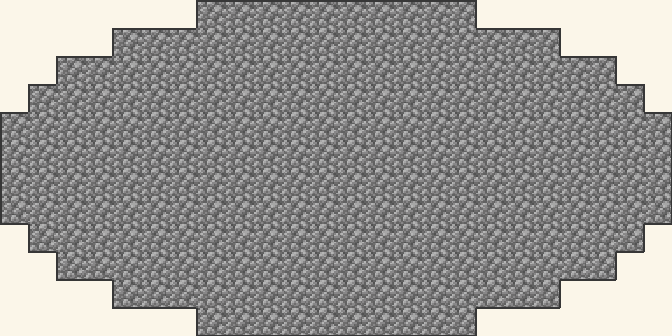
\includegraphics[width=0.45\textwidth]{fig07_2d_ellipse_24x12.png}
\caption{Ellipse $W = 24, H = 12$ in Block Round. Notice how cells along the major axis are more spaced than along the minor axis.}
\label{fig:elipse}
\end{figure}

\begin{enumerate}[leftmargin=1.5em,itemsep=0.15em,topsep=0.3em]
  \item Switch the shape to \acc{Ellipse}. Two \emph{sliders} appear: \emph{Width} and \emph{Height}.
  \item Set $W = 24$, $H = 12$. Observe the elongated shape --- see Figure~\ref{fig:elipse}.
  \item Discuss: \emph{\enquote{The equation governing this shape is $(x/12)^2 + (y/6)^2 = 1$. Why do we divide $x$ by $12$ and $y$ by $6$?}}
\end{enumerate}

\subsection{3D mode: sphere and ellipsoid}

\begin{enumerate}[leftmargin=1.5em,itemsep=0.15em,topsep=0.3em]
  \item Switch the mode to \acc{3D / Sphere}, size $D = 12$.
  \item Drag with the \emph{mouse} to rotate. A sphere of voxels appears.
  \item Activate the \emph{Info chip}: record the volume (\enquote{904 blocks $= 14 \times 64 + 8$}).
  \item Switch to \acc{Ellipsoid}, $W = 20$, $H = 10$, $D = 12$.
  \item Demonstrate the \emph{Cut slider} on the \texttt{Y} axis, 50\% (see Figure~\ref{fig:cortes}(a)). Observe the upper half disappear.
  \item Switch to the diagonal axis $\swarrow$/$\nearrow$ ($45^\circ$, Figure~\ref{fig:cortes}(c)). Discuss the oblique cut.
\end{enumerate}

\subsection{Export to Minecraft}
\begin{enumerate}[leftmargin=1.5em,itemsep=0.15em,topsep=0.3em]
  \item Show the \emph{download} button at the corner of the canvas: PNG.
  \item Show the \emph{export schematic} button: saves a \texttt{.schem} file in Sponge v2 format.
  \item Demonstrate (if possible) the import into Minecraft Java via the Litematica mod. See Appendix~\ref{ap:litematica}.
\end{enumerate}

% =============================================================================
\newpage
\section{Problem set}\label{ap:exerc}

\textbf{Instructions:} answer individually. You may consult Block Round to confirm answers, \emph{but mathematical justification is required}. Submit handwritten or typed.

\subsection*{Exercise 1 --- Equation of the circle}
\textbf{Problem:} Consider a circle centered at the origin $(0, 0)$ with radius $r = 7$. Decide whether each of the following points is \emph{inside}, \emph{outside}, or \emph{on} the circle. Justify with the equation.
\begin{enumerate}[label=\alph*),leftmargin=1.5em,itemsep=0.1em,topsep=0.2em,nosep]
  \item $(3, 4)$ \hfill \emph{answer:} inside ($9 + 16 = 25 < 49$).
  \item $(5, 5)$ \hfill \emph{answer:} \acc{outside} ($25 + 25 = 50 > 49$, since $\sqrt{50} \approx 7.07$).
  \item $(0, 7)$ \hfill \emph{answer:} on.
  \item $(-7, 0)$ \hfill \emph{answer:} on.
\end{enumerate}

\textit{Pedagogical note:} item (b) is a deliberate trap.

\subsection*{Exercise 2 --- Stack and chest arithmetic}
\textbf{Problem:} Consider a sphere $D = 8$ in the Euclidean algorithm, with continuous volume $V = \tfrac{4}{3}\pi \cdot 4^3 \approx 268.1$ and discrete volume $V_{\mathrm{disc}} = 268$.
\begin{enumerate}[label=\alph*),leftmargin=1.5em,itemsep=0.1em,topsep=0.2em,nosep]
  \item How many stacks of cobblestone are needed to build it? Answer in the form $q$ stacks $+$ $r$ extra blocks.
  \item How many single chests (27 slots) are needed to store all those stacks?
  \item In survival mode, assuming 1 block mined every 0.5 seconds with an iron pickaxe, what is the total collection time?
\end{enumerate}

\emph{Answer:} (a) $268 = 4 \times 64 + 12$, that is, \acc{4 full stacks $+$ 12 extra blocks} (5 inventory slots). (b) 1 single chest suffices (27 slots, only 5 used). (c) $268 \times 0.5 = 134$ seconds $\approx$ 2 min 14 s.

\subsection*{Exercise 3 --- Algorithm comparison for D=20}
\textbf{Problem:} In Block Round, generate a circle of diameter $D = 20$ in all three algorithms.
\begin{enumerate}[label=\alph*),leftmargin=1.5em,itemsep=0.1em,topsep=0.2em,nosep]
  \item Record the area (number of blocks) for each algorithm.
  \item Which algorithm minimizes material? Which maximizes?
  \item Difference in \emph{stacks} between largest and smallest? Is it worth choosing the smallest for economy?
\end{enumerate}

\emph{Expected answer:} Euclidean $\approx 316$ blocks (4 stacks $+$ 60 extra), Bresenham $\approx 316$, Threshold $\approx 332$ blocks (5 stacks $+$ 12 extra). Difference: $\approx 1$ stack. On large projects (spheres $D \geq 32$) the savings accumulate.

\subsection*{Exercise 4 --- Dome volume and storage}
\textbf{Problem:} Consider a sphere $D = 16$, Euclidean algorithm, cut in Y at 50\% (classic dome).
\begin{enumerate}[label=\alph*),leftmargin=1.5em,itemsep=0.1em,topsep=0.2em,nosep]
  \item Continuous volume of the full sphere.
  \item Volume of the dome (upper half).
  \item How many double chests are needed to store all the blocks for the dome?
  \item Is there leftover material to build part of the floor (a flat $16 \times 16$ block layer beneath the dome)?
\end{enumerate}

\emph{Answer:}
(a) $V = \tfrac{4}{3}\pi \cdot 8^3 \approx 2{,}144.66$, $V_{\mathrm{disc}} \approx 2{,}145$. (b) $V_{\mathrm{dome}} \approx 1{,}095$. (c) $\lceil 1{,}095 / 3{,}456 \rceil = 1$ double chest. (d) Leftover: $3{,}456 - 1{,}095 = 2{,}361$ blocks. Floor $16 \times 16 = 256$ blocks. $2{,}105$ blocks remain --- enough to build the floor plus a counter layer.

\subsection*{Exercise 5 --- Ellipsoid \enquote{giant round table}}
\textbf{Problem:} Consider an ellipsoid with $W = 24$, $H = 8$, $D = 24$ (flattened \enquote{table} shape).
\begin{enumerate}[label=\alph*),leftmargin=1.5em,itemsep=0.1em,topsep=0.2em,nosep]
  \item Continuous volume.
  \item Estimated discrete volume in Block Round.
  \item Leftover or shortage if you bought 3 double chests of Oak Planks?
\end{enumerate}

\emph{Answer:}
(a) $V = \tfrac{4}{3}\pi \cdot 12 \cdot 4 \cdot 12 \approx 2{,}413$.
(b) $V_{\mathrm{disc}} \approx 2{,}400$ (varies $\pm 10$ depending on algorithm).
(c) Purchased capacity: $3 \times 3{,}456 = 10{,}368$ blocks. Big leftover --- $\approx 8{,}000$ extra blocks. \emph{Overspending.} The ideal would have been 1 double chest (leftover of $\approx 1{,}000$ blocks).

\subsection*{Exercise 6 --- WorldEdit vs.\ Block Round}
\textbf{Problem:} The WorldEdit command \cmd{//sphere stone 15} uses an algorithm similar to Bresenham 3D. Compare it with the Block Round output in Bresenham mode with $D = 30$:
\begin{enumerate}[label=\alph*),leftmargin=1.5em,itemsep=0.1em,topsep=0.2em,nosep]
  \item Should they be identical?
  \item If not, why? List at least two reasons.
\end{enumerate}

\emph{Answer:}
(a) \emph{Approximately yes} --- both are Bresenham 3D, but (b) they may differ due to: (i) different implementations (Block Round is in JavaScript; WorldEdit is in Java); (ii) handling of diameter parity (even vs.\ odd); (iii) the empirical \emph{threshold} constant (if either internally uses Threshold). Typical difference: 0--6 blocks for $D = 30$.

\subsection*{Exercise 7 --- Construction by octahedral symmetry}
\textbf{Problem:} Plan the construction of a sphere $D = 16$ centered at $(0, 72, 0)$ in Minecraft, using symmetry. Build 1 octant (region $+x, +y, +z$, $\approx 268$ blocks) and reflect 7 times via \cmd{/clone}.
\begin{enumerate}[label=\alph*),leftmargin=1.5em,itemsep=0.1em,topsep=0.2em,nosep]
  \item Write the 7 \cmd{/clone} commands (use \cmd{mode:masked} to preserve existing terrain).
  \item Compute the total estimated time: manual octant construction + commands.
\end{enumerate}

\emph{Answer:}

\begin{minecraft}[Command sequence]
\cmd{/clone 0 72 0 7 79 7 -8 72 0 mode:masked} \quad (reflect.\ $-x$)\\
\cmd{/clone 0 72 0 7 79 7 0 64 0 mode:masked} \quad\quad (reflect.\ $-y$)\\
\cmd{/clone 0 72 0 7 79 7 0 72 -8 mode:masked} \quad (reflect.\ $-z$)\\
\cmd{/clone -8 72 0 -1 79 7 mode:masked} \quad\quad\;\; (octant $-x,-y$)\\
\cmd{/clone 0 64 -8 7 71 -1 mode:masked} \quad\quad\;\; (octant $-y,-z$)\\
\cmd{/clone -8 72 -8 -1 79 -1 mode:masked} \quad\;\; (octant $-x,-z$)\\
\cmd{/clone -8 64 -8 -1 71 -1 mode:masked} \quad\;\; (octant $-x,-y,-z$)
\end{minecraft}

Time: $\sim$\,5 min (manual octant in survival) + $\sim$\,3 s (7 clones).

\subsection*{Exercise 8 --- Final project}
\textbf{Problem:} After producing the group construction (Activity~\ref{at:53}), answer:
\begin{enumerate}[label=(\arabic*),leftmargin=1.7em,itemsep=0.15em,topsep=0.2em,nosep]
  \item List the geometric figures used (circle, ellipse, sphere, ellipsoid) and their parameters (diameter or semi-axes).
  \item For the main figure, which algorithm was chosen? Why? What visual effect does it produce that the other two would not?
  \item Were there 3D cuts? If so, describe \emph{one} of them mathematically as an inequality.
  \item How many stacks/chests would actually be required to build in Minecraft survival?
  \item Does your production engage with any American cultural reference (modernist art, geodesic architecture, Indigenous tradition, Mound Builder culture, Minecraft creator community)? Comment.
\end{enumerate}

% =============================================================================
\newpage
\section{Adaptation for schools without a computer lab}\label{ap:adapt-analog}

This adaptation allows the sequence to be applied \emph{entirely on paper} when computer access is unfeasible --- a frequent reality in rural Title I schools, Bureau of Indian Education (BIE) schools in remote locations, and some adult education programs. The conceptual axis remains intact; what changes is the material support.

\subsection{Substitutions by lesson}

\begin{center}
\small
\begin{tabularx}{\textwidth}{@{}p{0.13\textwidth}p{0.32\textwidth}X@{}}
\toprule
\textbf{Lesson} & \textbf{Original activity} & \textbf{Analog adaptation} \\
\midrule
1 & Block Round demonstration (1.3) & The teacher draws by hand three versions of the diameter-10 circle on a pre-printed grid the size of the board --- one per algorithm. Figures~\ref{fig:comp-d10} and~\ref{fig:comp-d20} can be printed as a reference. \\
\addlinespace[3pt]
2 & Quantitative software comparison (\ref{at:25}) & Distribute sheets with the three pre-drawn circles of $D = 16$ and ask for manual counting. \\
\addlinespace[3pt]
3 & 3D sphere generation (\ref{at:31}, \ref{at:32}) & Distribute sheets with \emph{slices} of the sphere ($z = 0, 1, 2, \ldots$) on graph paper. The student builds the mental model by stacking. Each sheet simulates a \emph{layer} of Minecraft blocks. \\
\addlinespace[3pt]
4 & Minecraft commands (\ref{at:42}) & Replace commands with \emph{construction instructions} written in English; students simulate execution on graph paper. \\
\addlinespace[3pt]
5 & Real Minecraft construction (\ref{at:53}) & Construction in \emph{LEGO} (if available), in graph paper colored with grass-green and dirt-brown pencils, or in \emph{paper cubes} folded by students in Art class. \\
\bottomrule
\end{tabularx}
\end{center}

\subsection{Helper handouts}
For the full analog version, prepare in advance:
\begin{itemize}[leftmargin=1.3em,itemsep=0.1em,topsep=0.2em,nosep]
  \item 1 A3/tabloid sheet with a $30 \times 30$ grid drawn by ruler.
  \item 1 set per student of 5 A4 (or 8.5x11 inch) graph-paper sheets (5 mm or 1/4 inch).
  \item 1 sheet with the three comparative circles pre-printed: Figures~\ref{fig:comp-d10} and~\ref{fig:comp-d20} in this plan, A4/letter size, serve as a reference.
  \item For analog Lesson 5: 8 pre-folded paper cubes per group (representing blocks of cobblestone, oak, quartz, diamond).
\end{itemize}

\subsection{Leveraging local knowledge}
In schools serving Indigenous students or in communities with strong artisanal traditions (Pueblo pottery in New Mexico and Arizona, Navajo weaving, Appalachian quilting, Acoma and Zuni ceramics, Anishinaabe Woodland Style art, Hopi katsina carving), Lesson~\ref{lesson3} can be \emph{enriched with a visit from traditional knowledge bearers}: potters, weavers, quilters, showing how they rasterize circles in their own languages. This approach realizes both the ethnomathematical principle and the state-level Indigenous-education frameworks such as Montana's \emph{Indian Education for All} and Washington's SB 5433.

% =============================================================================
\newpage
\section{Technical glossary for the teacher}\label{ap:glos}

\begin{itemize}[leftmargin=1.4em,itemsep=0.3em,topsep=0.3em]
  \item \acc{Algorithm} --- a finite, well-defined sequence of instructions for solving a problem. The three Block Round algorithms (cf.\ Figure~\ref{fig:comp-d10}) are distinct procedures for the same problem.
  \item \acc{AMC 10/12} --- American Mathematics Competitions, run by the Mathematical Association of America. Entry to AIME and USAMO.
  \item \acc{AP (Advanced Placement)} --- the College Board program offering college-level courses and exams to U.S. high school students. AP Calculus AB/BC and AP Precalculus are directly relevant here.
  \item \acc{Block} --- the construction unit of Minecraft. A $1\times1\times1$ cube with six textured faces. In mathematical terms, a \emph{voxel}.
  \item \acc{Bresenham (algorithm of)} --- algorithm published in 1965 by Jack Bresenham (IBM), originally for line drawing, later extended by Pitteway and others to ellipses. Its hallmark is using \emph{integers only}. See Activity~\ref{at:23}.
  \item \acc{Canvas} --- HTML element that provides a 2D or 3D drawing area in the browser.
  \item \acc{CCSS} --- Common Core State Standards. The national mathematics standards adopted in 2010 by most U.S. states.
  \item \acc{Chest (single)} --- Minecraft container with 27 slots. Capacity: $27 \times 64 = 1{,}728$ items.
  \item \acc{Chest (double)} --- two adjacent chests merged into a 54-slot container. Capacity: $54 \times 64 = 3{,}456$ items.
  \item \acc{\code{/clone}} --- vanilla Minecraft command that copies a rectangular region to another position. Syntax: \cmd{/clone x1 y1 z1 x2 y2 z2 dx dy dz}. Essential for symmetric construction.
  \item \acc{CTE} --- Career and Technical Education. The U.S. high school pathway program funded by the Carl D. Perkins Act.
  \item \acc{Ethnomathematics} --- field of study founded by Brazilian mathematician Ubiratan D'Ambrosio and developed in the U.S.\ by Marcia Ascher.
  \item \acc{FERPA} --- Family Educational Rights and Privacy Act (1974). Federal U.S.\ law governing student record privacy.
  \item \acc{\code{/fill}} --- vanilla Minecraft command that fills a rectangular box with a given block type. Syntax: \cmd{/fill x1 y1 z1 x2 y2 z2 minecraft:stone}.
  \item \acc{Implicit equation} --- an equation of the form $F(x, y) = 0$. The ellipse: $(x/r_x)^2 + (y/r_y)^2 - 1 = 0$.
  \item \acc{IAS} --- Institute for Advanced Study (Princeton, NJ). One of the foundational mathematical-research institutes of the U.S.
  \item \acc{Litematica} --- popular Minecraft Java Edition mod that imports schematics and shows a translucent \emph{ghost} of the construction to be built block by block. Free.
  \item \acc{Minecraft Education Edition} --- educational version of Minecraft, free for licensed K--12 schools through Microsoft Education.
  \item \acc{NCTM} --- National Council of Teachers of Mathematics. The principal professional organization for U.S.\ math teachers.
  \item \acc{Pack / Stack} --- a stack of up to 64 identical blocks in a Minecraft inventory slot.
  \item \acc{Pixel} --- short for \emph{picture element}. In 2D.
  \item \acc{PWA} --- \emph{Progressive Web App}. Web application that is installable and operable \emph{offline}.
  \item \acc{Rasterization} --- the process of converting a continuous geometric description into a matrix of pixels (2D) or voxels (3D).
  \item \acc{Schematica} --- alternative mod to Litematica, with similar function.
  \item \acc{Schematic (\texttt{.schem})} --- file format that serializes a Minecraft region (Sponge Schematic v2, gzip + NBT).
  \item \acc{Semi-axis} --- in an ellipse, the distance from the center to the endpoint along the axis direction.
  \item \acc{\code{//sphere}} --- WorldEdit command that builds a sphere. Syntax: \cmd{//sphere block radius}.
  \item \acc{Slot} --- individual cell in the Minecraft inventory. Full player inventory: 36 slots ($9 \times 4$).
  \item \acc{USACO} --- USA Computing Olympiad.
  \item \acc{Voxel} --- short for \emph{volume element}. The 3D generalization of the pixel. In Minecraft, each \emph{block} is a voxel.
  \item \acc{WebGL} --- 3D graphics programming library for browsers.
  \item \acc{WorldEdit} --- highly popular Minecraft Java mod that adds advanced large-scale construction commands, including \cmd{//sphere}, \cmd{//hsphere}, \cmd{//ellipsoid}, \cmd{//cyl}, \cmd{//schem load}.
\end{itemize}

% =============================================================================
\newpage
\section{Tutorial: from Block Round to Minecraft via Litematica}\label{ap:litematica}

This appendix describes the full flow of export from Block Round and import into Minecraft Java Edition using the \emph{Litematica} mod. Expected total time: 15 minutes (first time).

\subsection{Prerequisites}
\begin{itemize}[leftmargin=1.3em,itemsep=0.1em,topsep=0.2em,nosep]
  \item Minecraft Java Edition (purchase at the \emph{Mojang Store}; \emph{Minecraft Education} also works, with adjustments).
  \item \emph{Fabric Loader} for the Minecraft version you use (usually the latest: \url{https://fabricmc.net/use/}).
  \item Mods: \emph{Fabric API} and \emph{Litematica} (\url{https://www.curseforge.com/minecraft/mc-mods/litematica}).
  \item Block Round open in your browser, with the desired figure already produced.
\end{itemize}

\subsection{Step 1: export from Block Round}
\begin{enumerate}[leftmargin=1.5em,itemsep=0.15em,topsep=0.3em]
  \item In Block Round, configure the desired figure (mode, shape, diameter, algorithm, block, cut). Check the volume in the \emph{Info chip}.
  \item Click the \emph{Export Schematic} button (upper-right corner of the canvas, second icon). A \texttt{.schem} file will download.
\end{enumerate}

\subsection{Step 2: install Litematica}
\begin{enumerate}[leftmargin=1.5em,itemsep=0.15em,topsep=0.3em]
  \item Install Fabric Loader for the Minecraft version you use.
  \item Download \emph{Fabric API} and \emph{Litematica} for the same Minecraft version. Place both in the \texttt{.minecraft/mods/} directory.
  \item Launch Minecraft with the \emph{fabric-loader-x.y.z-1.20.x} profile.
\end{enumerate}

\subsection{Step 3: import the schematic}
\begin{enumerate}[leftmargin=1.5em,itemsep=0.15em,topsep=0.3em]
  \item Place the \texttt{.schem} file in \texttt{.minecraft/schematics/} (or in the default folder defined in Litematica settings).
  \item In a world (creative or survival), press \texttt{M} to open the Litematica menu.
  \item Click \emph{Load Schematic} $\rightarrow$ select the file $\rightarrow$ \emph{Load}.
  \item The schematic now appears in a list. Click it and \emph{Placement}: the translucent \enquote{ghost} of the figure appears in the world.
  \item Use movement controls (\texttt{M} $\rightarrow$ \emph{Placements}) to drag the ghost to the desired position. For flat terrain, simply position the bottom corner $(x_1, y_1, z_1)$ on the ground.
\end{enumerate}

\subsection{Step 4: build}
\begin{enumerate}[leftmargin=1.5em,itemsep=0.15em,topsep=0.3em]
  \item In \emph{Creative}: fly over the ghost and place each block where Litematica shows; the mod confirms correct blocks in green and marks any error in red. Building a $D = 12$ sphere takes $\approx$\,5 minutes.
  \item In \emph{Survival}: identical, but you must gather the blocks first. Use the stack/chest calculation from Activity~\ref{at:41} to plan collection.
  \item Alternative: if the server has WorldEdit, use \cmd{//schem load filename} followed by \cmd{//paste -a} for instant construction.
\end{enumerate}

\subsection{Step 5: verification}
Litematica highlights in red any block that is wrong (missing, wrong type, or wrong position). Use the \texttt{Z} shortcut to toggle between \emph{visible} and \emph{invisible} ghost, comparing with the actual build.

\subsection{Common troubleshooting}
\begin{itemize}[leftmargin=1.3em,itemsep=0.15em,topsep=0.3em,nosep]
  \item \emph{Schematic does not appear in the list:} check that the file is in the correct folder, and that the Litematica version matches the Minecraft version.
  \item \emph{Wrong/gray blocks:} some blocks in Block Round schematics may be unavailable in your world (older Minecraft version); open the schematic with a text editor to check names.
  \item \emph{Ghost floats:} adjust the position with the \emph{Rotation/Mirror} option in the Placement menu. For spheres, it is indifferent; for ellipses, adjust rotation.
\end{itemize}

\vspace{2em}
\begin{center}
\color{muted}\small\sffamily
--- end of lesson plan ---
\end{center}

\end{document}
